% This is LLNCS.DOC the documentation file of
% the LaTeX2e class from Springer-Verlag
% for Lecture Notes in Computer Science, version 2.4
\documentclass{llncs}
\usepackage{llncsdoc}
\usepackage[hyphens]{url}
\usepackage[pdftex]{graphicx}     
\usepackage{float}
\usepackage{tablefootnote}
\usepackage{hyperref}

\hyphenation{block-chain}

	%%%%%%%%%%%%%%%%%%%%%%%55
	%% Added to enable numbering for subsubsections, otherwise they would look like paragraphs which is ugly
	%%%%%%%%%%%%%%%%%%%%%%%55
	
	\makeatletter
	\renewcommand\subsubsection{\@startsection{subsubsection}{3}{\z@}%
		{-18\p@ \@plus -4\p@ \@minus -4\p@}%
		{0.5em \@plus 0.22em \@minus 0.1em}%
		{\normalfont\normalsize\bfseries\boldmath}}
	\makeatother
	\setcounter{secnumdepth}{3}

%
\begin{document}


	{
	%
	\title{Enabling the Vehicle Economy Using a Blockchain-Based Value Transaction Layer Protocol for Vehicular Ad-Hoc Networks\\ \small Research Paper - Version 0.3\\\small \today}
	
	\author{Benjamin Leiding \and Will Vorobev}
	
	\institute{ 
		Chorus Technology\\
		Email: hello@chorus.technology\\
		Website: chorus.technology	
	}
	
	\maketitle

	%% ----------------------------------------------------------------
	%% ----------------------------------------------------------------

	\begin{abstract}

		% A good abstract:
		%1.) What is the paper about?
		%2.) What is the SoA?
		%3.) What is the detected gap?
		%4.) What are the main questions to be answered pertaining to the gap?
		%5.) Why is the solution good/better than other solutions?

		The next generation of tightly interconnected vehicles offers a variety of new technological as well as  business opportunities. Vehicles form so called vehicular ad-hoc networks (VANETs) in order to enable vehicle-to-vehicle (V2V), vehicle-to-infrastructure (V2I), vehicle-to-human (V2H), or in general vehicle-to-everything (V2X) communication and interaction. A variety of manufacturers started implementing specific use cases that are limited to their own products. However, a default interaction standard for this new economy is still missing. Chorus Technology presents a blockchain-based system that enables a manufacturer agnostic platform solution that allows VANET participants to enact and transact any kind of provision of service and goods. This whitepaper fills the gap in the state of the art by introducing a blockchain-based transaction layer library for (semi)-autonomous vehicles that enables the upcoming V2X economy. We present the advantages of the system, outline the requirements and goals, as well as the architecture of the Chorus V2X platform and eco-system. In addition, we present a Chorus Technology prototype that demonstrates how our system can help mitigating traffic jams and at the same time provides a mean to car insurance companies to incentivize their customers to practice good driving behavior.
 


	\end{abstract}
	
	
	\keywords{Blockchain, Autonomous Vehicles, V2X Communication, Chorus Technology, Self-Driving Cars, VANET, Smart Contract}

	%% ----------------------------------------------------------------
	%% ----------------------------------------------------------------
	
	\section{Introduction}
		\label{s:introduction}

		Despite steadily growing public transport networks and systems, especially in most first world countries, cars and similar vehicles are still the default standard for urban transportation. In the US, ``about 86 percent of all workers commuted to work by private vehicle, either driving alone or carpooling" \cite{mckenzie2015drives} even though in recent years the numbers remained relatively stable after decades of consistent increase - similar applies to other industrial countries \cite{netherlandsPublicTransport}\cite{zealand2006car} even though the overall percentage of vehicle commuters in Europe is lower than in the US \cite{commuteUSvsEurope}. While it was normal for the last few decades to own a vehicle and commute on a day-by-day basis, the future will be radically different due to the progressing evolution of self-driving cars and autonomous vehicles. The car-sharing economy that developed in recent years in combination with autonomous cars results in a so called \textit{passenger economy} \cite{intelPassengerEconomy}. Users no longer own cars, instead just hop on an autonomous cars, pick a destination and get delivered without any human interaction. An Intel report estimates the size of this economy to be around US\$ 7 Trillion in 2050 \cite{intelPassengerEconomy}.
		
		Despite some recent setback, e.g. Uber and Tesla accidents \cite{bibid}\cite{bibid}\cite{bibid}, academic researchers as well as companies from the private sector make fast progresses in the research area of self-driving cars \cite{bibid}\cite{bibid}. It took less than 15 years from the first DARPA Grand Challenge (a prize competition for autonomous vehicles) to self-driving cars operating on public streets on a regular base (Tesla, Waymo, Uber, etc.) \cite{bibid}\cite{bibid}\cite{bibid}. Besides the cars, several projects are also already working on system solutions for trucks, rovers, drones, ships and even airplanes \cite{bibid}\cite{bibid}\cite{bibid}\cite{davWhitepaper}. But progressing automation and driverless transport that enables the passenger economy is only a small aspect of the potential of these new technologies. During a talk\footnote{\url{https://www.youtube.com/watch?v=MVyv4t0OKe4}} at the 2013 Turing Festival in Edinburgh, Mike Hearn did not only described a vision where most users don't own cars anymore and instead use services provided by autonomous vehicles that own itself, but also the potentials of a vehicle-to-vehicle (V2V) as well as a vehicle-to-infrastructure (V2I) economy. Autonomous vehicles (AVs) may own themselves, offer services and goods to earn money, and pay money to acquire services that they cannot provide on their own, e.g., car renting a parking lot, paying for a charged battery, using toll roads, or simple service check ups. The idea of V2V and V2I or in general V2X (vehicle-to-everything) will fuel various new business fields. 
		
		Certainly, traditional payment systems such as paper money or fiat currencies in general are not suited to be part of this new economy. There are slow, depend on third parties (e.g., banks) and suffer from bureaucratic overhead. Blockchain technology and cryptocurrencies offer a promising alternative payment solution that comes with several additional advantages that we will discuss later on. The blockchain technology, also referred to as distributed ledger system, is most noticeably known for providing the foundation of the peer-to-peer (P2P) cryptocurrency and payment system Bitcoin \cite{nakamoto_bitcoin:2008}, but nowadays there a various different platforms out there, e.g., \cite{tezosWhitepaper}\cite{iotaWhitepaper}\cite{wood2014ethereum}. Several companies already started to prototype applications that combine vehicles and blockchains. Porsche is researching different payment-related applications for vehicles \cite{porscheBlockchain} whereas Ford focuses on traffic marshaling \cite{macneille2018vehicle}. As expected in the early days of a new technology, companies focus on selective solutions for a selection of very specific problems or use cases and the resulting solutions are only compatible with their own products. What is currently missing in the new business field of V2X economy is an industry standard that can easily be integrated with self-driving and (semi)-autonomous cars or even nowadays cars. 

%https://www.heise.de/newsticker/meldung/Dubai-will-smarte-Kfz-Kennzeichen-testen-4016538.html

%%%%%%%%%%%%%%%%%%%%%%%%%%%%%%%%%%%%%%%%%%%%%%%%%%%%%%%%%%%%%%%%%%%%%%

%		RQ: How to implement a blockchain-based transaction layer library for (semi)-autonomous vehicles that enables a V2X platform for goods and services?
%		RQ-1: What is the long term vision of Chorus Technology?
%		RQ-2: What are the critical requirements and the corresponding architecture of the Chorus platform?
%		RQ-3: What are the system-engagement processes for the stakeholders?


%%%%%%%%%%%%%%%%%%%%%%%%%%%%%%%%%%%%%%%%%%%%%%%%%%%%%%%%%%%%%%%%%%%%%%

		This whitepaper addresses the detected gap by introducing the Chorus Technology solution, thereby answering the question of how to implement a blockchain-based transaction layer library for (semi)-autonomous vehicles that enables a V2X platform for goods and services? In order to answer this question with a separation of concerns, we pose the following sub-questions: What is the long term vision of Chorus Technology? What are the critical requirements and the corresponding architecture of the Chorus platform? What are the system-engagement processes for the stakeholders?

		The remainder of this paper is structured as follows: Section~\ref{s:section-2} introduces supplementary literature and related work. Section~\ref{s:section-3} then outlines the vision of Chorus Technology as well as different use-cases. Afterwards, Section~\ref{s:section-4} analyses the requirements of the our system and outlines the resulting system architecture that we derive from the requirements. Afterwards, Section~\ref{s:section-5} expands on the system-engagement processes for the stakeholders, followed by Section~\ref{s:section-6} that introduces the Chorus prototype as well as feasibility evaluation. Section~\ref{s:section-7} provides an discussion and an analysis of related projects. Finally, Section~\ref{s:section-8} concludes this work and provides an outlook on future work.


	%% ----------------------------------------------------------------
	%% ----------------------------------------------------------------

	\section{Technical Background and Supplementary Literature}	
		\label{s:section-2}
		
		The following section provides background information and describes related works regarding previous ideas and concepts that focus on a blockchain-based VANET platforms. First, Section~\ref{ss:blockchain-intro} introduces the general concepts of blockchain technology, terms and frameworks. Afterwards, Section~\ref{ss:autonomous-vehicles} and Section~\ref{ss:vanets} focus on the fundamentals of autonomous vehicles as well as vehicular ad-hoc networks. %Finally, Section~\ref{ss:traffic-wave-theory} introduces traffic waves, flows and congestions. 
					
		%% ----------------------------------------------------------------
		%% ----------------------------------------------------------------	
		
		\subsection{Blockchain Technology}
			\label{ss:blockchain-intro}
			
			As the name suggests, a blockchain consists of a chronologically ordered chain of blocks. Every block consists of a certain number of validated transactions and each of those block links to its predecessor by a hash reference. As a result, changing the content of one block also changes all succeeding blocks and hence breaks the chain. All blocks are stored on and verified by all participating nodes. While the initial Bitcoin blockchain only supported a very limited set of scripting instructions, the next generation of blockchain platforms, e.g., Ethereum \cite{wood2014ethereum}, Qtum \cite{qtumWhitepaper}, or Tezos \cite{tezosWhitepaper}, provide Turing-complete programming languages on the protocol-layer level in order to enable smart contract capabilities. Smart contracts are, ``orchestration- and choreography protocols that facilitate, verify and enact with computing means a negotiated agreement between consenting parties" \cite{qtumWhitepaper}. Hence, the parties participating in the enactment of a smart contract establish binding agreements and deploy applications using such smart contracts in order to provide blockchain-based applications. Those application are as versatile as smart contracts itself and enable services including the finance sector \cite{nguyen2016blockchain}\cite{saltWhitepaper}, academic and business authentication and identity solutions \cite{leidingUnchained}\cite{CivicWhitepaper}\cite{AuthcoinLeiding2016MCIS}\cite{mccorry2015authenticated}\cite{SelfkeyWhitepaper}, reputation systems \cite{SemadaWhitepaper} as well platforms for Internet-of-Things (IoT) applications \cite{christidis2016blockchains}\cite{ouaddah2017towards}. 	
			
			The blockchain concept is particularly interesting for the V2X economy for three reasons. First, it removes the need for trusted third parties and instead enables trust-less transaction enactment. Second, transactions that were agreed up on cannot be changed any more since the underlying blockchain is tamperproof. Third, no human interaction is required for any kind of transaction between vehicles or machines in general.

		%% ----------------------------------------------------------------
		%% ----------------------------------------------------------------	
		
		\subsection{Autonomous Vehicles}
			\label{ss:autonomous-vehicles}
			
			During the last 15 years research on autonomous and self-driving cars progressed a lot and nowadays such cars already operating on public streets on a regular base, e.g., Tesla, Waymo, Uber, and so on. The ultimate goal of most manufacturers and researchers is to develop the first fully self-driving and autonomous vehicle. In order to clarify some definitions, this short section provides a short introduction to the most relevant terms and concepts.

			An autonomous car, also referred to as a driverless car or robotic car, is able to navigating and interact with its environment without human input based on information provided by its sensors \cite{gehrig1999dead}\cite{thrun2010toward}. To do so, modern cars are equipped with radar- and laser sensors, lidars, GPS devices, cameras and several further sensing devices. Based on these information, the vehicle interprets the surrounding world and deduces appropriate action strategies such as avoiding obstacles (other vehicles, humans or a house) on the way to the supermarket \cite{dokic2015european}\cite{zhu2014vehicle}. As the technology developed over time, vehicles were equipped with more and more sensors, resulting in different driving capabilities. The SAE \cite{autonomyLevelsSAE}
			defined six levels of driving autonomy to categorize the varying capabilities and progresses of several approaches:		
			
			\begin{itemize}
				\item \textbf{Level 0 (No automation): }No driving autonomy, the driver has to perform all driving tasks and interactions.
				\item \textbf{Level 1 (Driver assistance): }The vehicle is controlled by the driver, but is supported by some basic driver assistance functionalities.
				\item \textbf{Level 2 (Partial automation): }The vehicle is able to perform some specific tasks (acceleration or steering) without driver input. Nevertheless, the driver must be fully engaged in driving task and monitor all decision of the car and the environment at all time. The user has to be able to intervene at any given moment. 
				\item \textbf{Level 3 (Conditional automation): }The driver is still a necessity, but is not required to monitor the vehicle or the environment at any given moment. But given a notification by the vehicle, the driver has to be able to take back control over the car in case the vehicle encounters a situation that it cannot deal with on its own.
				\item \textbf{Level 4 (High Automation): }The vehicle is able to perform all driving tasks without human intervention in most driving scenarios. The driver can take control whenever desired.
				\item \textbf{Level 5 (Full Automation): }The vehicle is able to perform all driving tasks without human intervention in all driving scenarios. The driver can take control whenever desired as long as a steering wheel is still part of the vehicle.
			\end{itemize}
			
			The Chorus interaction- and transaction layer library supports and enables a varying number of services for vehicles of each automation level, whereas the most sophisticated applications require SAE level 5 and simpler plug-ins may only require SAE level 0.

		%% ----------------------------------------------------------------
		%% ----------------------------------------------------------------	
		
		\subsection{Vehicular Ad-Hoc Networks - VANETs}
			\label{ss:vanets}

			Communication between vehicles, road infrastructure and Internet-based services is a key enabler of upcoming generation of vehicles. So called vehicular ad-hoc networks provide an abstract concept that models the different components that are required for V2V, V2I and V2X communication. As illustrated in Figure \ref{fig:vanets}, the basic components of VANETs are vehicles, on-board-units (OBUs), application-units (AUs) and road-side-units (RSUs).\\
			RSUs are placed  along the road side or in dedicated locations such as at crossroads. Usually, RSUs provide short range communication based on IEEE 802.11p radio technology but can also be equipped with other network devices in order to provide communication within the infrastructural network \cite{al2014comprehensive}. An OBU is typically mounted onto a vehicle and used for exchanging information with RSUs or other OBUs. Short range wireless communication or other radio technologies are usually used to exchange information \cite{baldessari2007car}.\\
			Closely linked to the OBU is the AU. They might even reside in the same physical unit or is mobile and might be regularly removed from the vehicle (e.g smartphones). The AU provides an execution environment for applications that utilize the OBU's communication capabilities \cite{al2014comprehensive}\cite{baldessari2007car}.\\	
			\begin{figure}[ht]
				\centering
				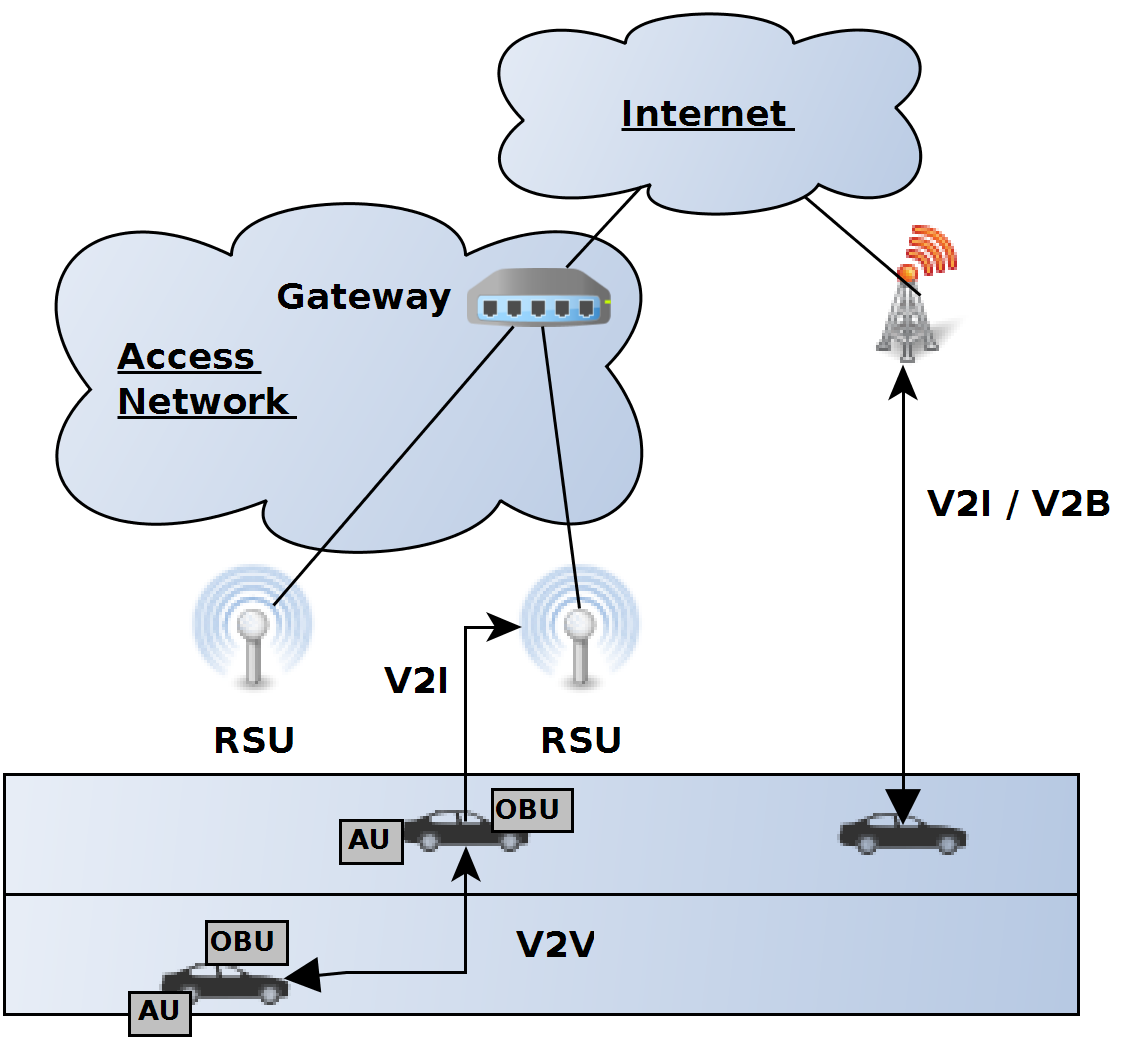
\includegraphics[scale=0.2]{Figures/Vanets.png}
				\caption{General VANET architecture (Based on: \protect\cite{baldessari2007car} and \cite{leiding2016self})}
				\label{fig:vanets}
			\end{figure}			
			Communication in VANETs occurs either inside a vehicle between AUs and OBU, wirelessly between different vehicles (V2V), vehicles and infrastructure (V2I) or vehicles and the infrastructure via broadband (V2B) \cite{faezipour2012progress}. For authentication purposes, each network participant is equipped with a unique public/private key pair which usually resides in a tamper-proof-device (TPD). In blockchain terms, the TPD is similar to an external hardware wallet.
			
		%% ----------------------------------------------------------------
		%% ----------------------------------------------------------------	
		

	%% ----------------------------------------------------------------
	%% ----------------------------------------------------------------

	\section{The Chorus Vision}
		\label{s:section-3}
		
		%%RQ-1: What is the long term vision of Chorus Technology?
		
Our end goal is to enable vehicles to own themselves and transact with each other as decentralized autonomous agents utilizing the latest break-through technologies within Blockchain and IoT ecosystems.		
		
%		Intro
%
%		We are focused on the research and development of the blockchain based peer-to-peer payments protocols and decentralized applications for driverless vehicles of tomorrow. Our end goal is to enable vehicles to own themselves and transact with each other as decentralized autonomous agents utilizing the latest break-trough technologies within Blockchain and IoT ecosystems.
%		
%		Areas Of Research
%			
%			DApps Development
%				User friendly and Blockchain-ready native mobile applications
%
%			Blockchain
%				Ethereum Blockchain Protocols for Ridesharing, Autonomous Vehicles, Road Space Negotiation
%				
%			Off-Chain
%				Ethereum Off-chain Protocols Implications for Instant Payments to and from Decentralized Agents
%			
%			Hardware
%				In-Car Hardware Nodes and HSM Wallets Engineering	
%
%			Mapping
%				Mapping and Cartography solutions on Blockchain
%
%			Communications
%				Wireless Communications and Geospatial Solutions for Autonomous Vehicles
%
%			Ethereum Scaling
%				Contribution to Plasma and Ethereum Sharding R\&D to scale for a real world use.

		%foam and localization somewheere here	
				

		%% ----------------------------------------------------------------
		%% ----------------------------------------------------------------	
		
		\subsection{Use Cases}
			\label{ss:use-cases}

			\textbf{Work-In-Progress}
			
%			CHECK THE chorus website for this section
%			
%			traffic wave fixing as one of the major selling points in the prototype as well as the main product
%			insurance example as a running case later for the prototype
		%% ----------------------------------------------------------------
		%% ----------------------------------------------------------------	
		
			
			
		\subsection{Vehicle to Human}
			\label{ss:V2H}
			
%			Decentralized Autonomous Taxi Haling and Sharing. We envision safe and seamless transactions with autonomous taxis. At the advent of autonomous taxis the Ethereum protocol will evolve to meet the security and trustless environmental needs for all types of ridesharing methods. This includes pooling, and sharing or splitting payments between multiple passengers within a single party.
%			
			
		%% ----------------------------------------------------------------
		%% ----------------------------------------------------------------	
		
		
		\subsection{Vehicle to Vehicle}
			\label{ss:V2V}
%			Decentralized peer-to-peer road space negotiation and payments. Traffic optimization incentive systems. In the future autonomous vehicles will need their own extremely secure and trustable network protocol through which to interact with one another. To combat congestion and increase the efficiency of traffic this system will prioritize traffic based on economic levers allowing self-driving cars to negotiate lane space.
%			
%			road space negotiation

%		\subsection{Traffic Flows, Traffic Congestions and Traffic Wave Theory}
%		\label{ss:traffic-wave-theory}
%		
%		In mathematics and civil engineering, traffic flow is the study of interactions between travellers (including pedestrians, cyclists, drivers, and their vehicles) and infrastructure (including highways, signage, and traffic control devices), with the aim of understanding and developing an optimal transport network with efficient movement of traffic and minimal traffic congestion problems.
%		
%		
%		multi-lane traffic flow \cite{daganzo2002behavioral}
%		Application of traffic-wave theory in urban traffic analysis \cite{wang2001application}
%		
%		adaptive cruise control design for active congestion avoidance\cite{kesting2008adaptive}
%		
		
		%% ----------------------------------------------------------------
		%% ----------------------------------------------------------------	
		
			
		\subsection{Vehicle to Infrastructure}	
			\label{ss:V2I}
							
%			Decentralized and Instant V2X (Vehicle to Anything) Payments. Paying per second when using a paid priority lane. Automatic toll payments by Autonomous Vehicles and Regular Taxis .
%		
		
		%% ----------------------------------------------------------------
		%% ----------------------------------------------------------------	


	%% ----------------------------------------------------------------
	%% ----------------------------------------------------------------
	
	
	\section{System Design and Architecture}
		\label{s:section-4}	

		%%RQ-2: What are the critical requirements and the corresponding architecture of the Chorus platform?

		The vision of Chorus outlined in Section \ref{s:section-3} is now analyzed from technical perspective as part of the following section. In order to identify, structure and formalize the critical requirements and stakeholders on an abstract level, we use one part of an Agent-Oriented Modeling (AOM) method \cite{sterling2009art}, i.e., goal models. Section~\ref{ss:requirement-engineering} introduces AOM goal models and the Chorus specific goal model. The produced goal model is used in subsequent Section \ref{ss:component-diagrams} to derive the Chrous system architecture . The resulting system architecture and specifications serve as implementation guidelines. 
		%Finally, Section~\ref{ss:smart-contract-lifecycle-management} provides some details on the smart contract lifecycle management within our solution, whereas Section~\ref{ss:library-api} outlines a general outlook on the APIs and how to integrate the Chorus library into external applications.
		
		
		%% ----------------------------------------------------------------
		%% ----------------------------------------------------------------	
		
		\subsection{Functional Goals, Quality Goals, Stakeholders and Requirements}
			\label{ss:requirement-engineering}
						
			In system development and software engieerng, good requirements follow certain characteristics. According to \cite{davis1993software}\cite{ieee1994ieee} requirements address one issue only and are completely specified without missing information. Moreover, they have to be consistent and do not contradict itself, or in correlation with other requirements. Finally, a requirement must also be atomic and without conjunctions \cite{norta2014reference}.

			\begin{figure}[H]
				\centering
				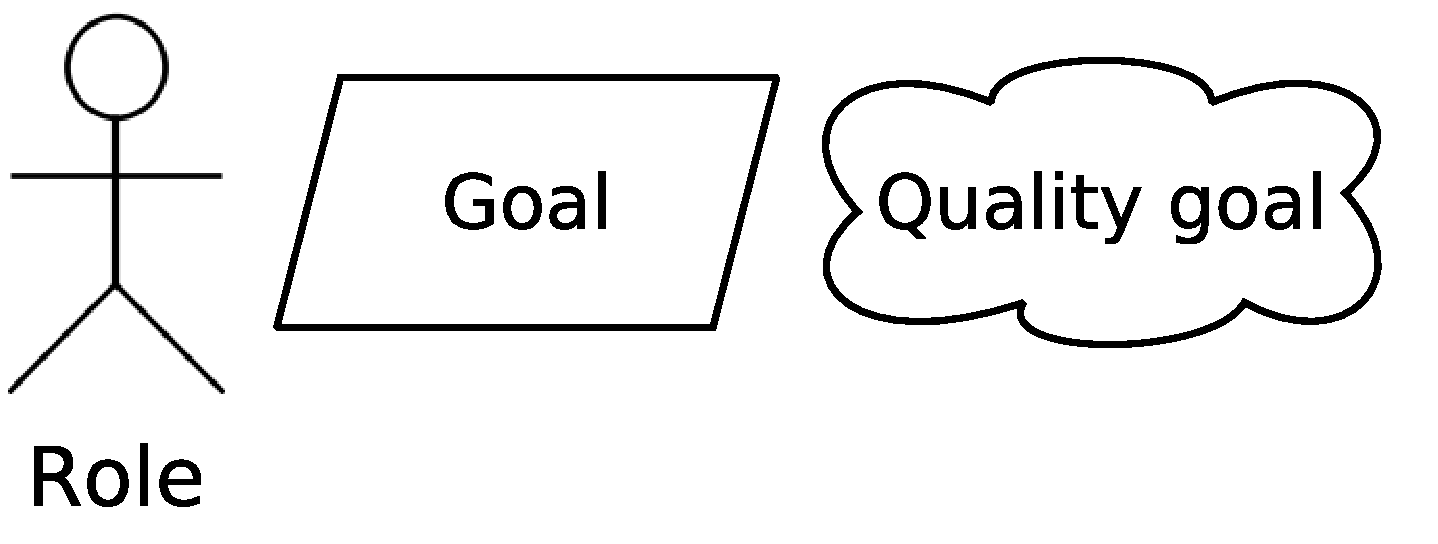
\includegraphics[scale=0.2]{Figures/20180426_AOM-notation.pdf}
				\caption{Selection of AOM notation elements.}	
				\label{fig:aom-notaion-elements}
			\end{figure}				
			The AOM methodology is a socio-technical requirements-engineering approach used to model complex systems that consist of humans, devices, and software agents. An AOM goal model enables both, technical- and non-technical stakeholders, to capture and understand the functional- and non-functional requirements of a complex system. Figure \ref{fig:aom-notaion-elements} depicts the three main elements that an AOM goal model comprises in order to capture the system requirements and goals. Roles of involved entities are represented in form of sticky men, whereas functional requirements are depicted as parallelograms. Note that in the specific context of this whitepaper, a sticky man does not exclusively represent human entities but rather all kinds of entities, e.g., also vehicles or infrastructure. Functional requirements are also referred to as goals. Non-functional requirements are depicted as clouds and refer to quality goals of the modeled software system. The AOM goal model follows a tree-like hierarchy with the root value proposition of the modeled system at the top. Subsequently, this main goal is decomposed into sub-goals where each sub-goal represents an aspect for achieving its parent goal \cite{marshall2014agent}. The goals are further decomposed into multi-layered sub-goals until the lowest atomic level is reached. Additionally, roles and quality goal may be assigned to goals and are inherited to lower-level goals. The following Section~\ref{sss:top-level-goal-model} introduces the top-level goal model our system, followed by Section~\ref{sss:quality-goals} focusing on the non-functional goals of the AOM goal model.

			
			%% ----------------------------------------------------------------
			%% ----------------------------------------------------------------	
					
			\subsubsection{Top-Level AOM Goal Model}
				\label{sss:top-level-goal-model}
				
				The presented AOM goal model is similar to the model presented by the authors in \cite{leidingM2M}, since implementation of a V2X system is a specific use case of the more abstract and general M2M (machine-to-machine) interaction platform represented in that paper. Meanwhile, Figure \ref{fig:top-level-aom-goal-model} presents the top-level AOM goal model of the system using the modeling method described above. The main value proposition is to provide a V2X interaction and transaction layer library for (autonomous) vehicles, thereby representing the root of the goal model. The complex main value proposition is split into four sub-goals representing the four main components.
				
				First, one component for managing the V2X platform. This functional goal includes managing certain aspects of the platform itself, e.g., creating, updating, deleting a new platform, as well as the management of the underlying smart contracts. Each platform operates a master smart contract and several sub-smart contracts. While the master contract is in charge of platform management and controlled by the hardware vendor (e.g., Tesla), the sub contracts each offer service provision for a specific service, interaction, transaction or application.
				
				The second functional goal enables V2X interaction. That mostly covers on- and off-chain supply and demand administration. Entities may register offers or requests on-chain in order to attract business partners, but for the other use cases a local supply demand management off-chain is more suitable, e.g., road-space negotiation. Supervising on- and off-chain auctions is basically equivalent to the on- and off-chain supply and demand management. Besides that, plug-ins and dApps of the Chorus eco-system might use platform smart contracts for service enactment and have to be integrated as well in this context.
				
				The third functional requirement, that represents the third main component, enables V2X transaction via the blockchain. The most important part here is the transaction management via a smart contract lifecycle that will be detailed later on in Section \ref{ss:smart-contract-lifecycle-management}.
				
				Finally, the fourth functional requirement focus on the enactment of various plug-ins and decentralized applications (dApps). Applications and plug-ins have to be registered, prepared for enactment, executed and terminated. Moreover, they have to interact with various entities of the eco-system depending on the use case. Since nowadays most blockchains offer Turing-complete smart contract support, the variety of applications and plug-ins in our eco-system is quite vast. 
				
%				\begin{figure}[H]
%					\centering
%					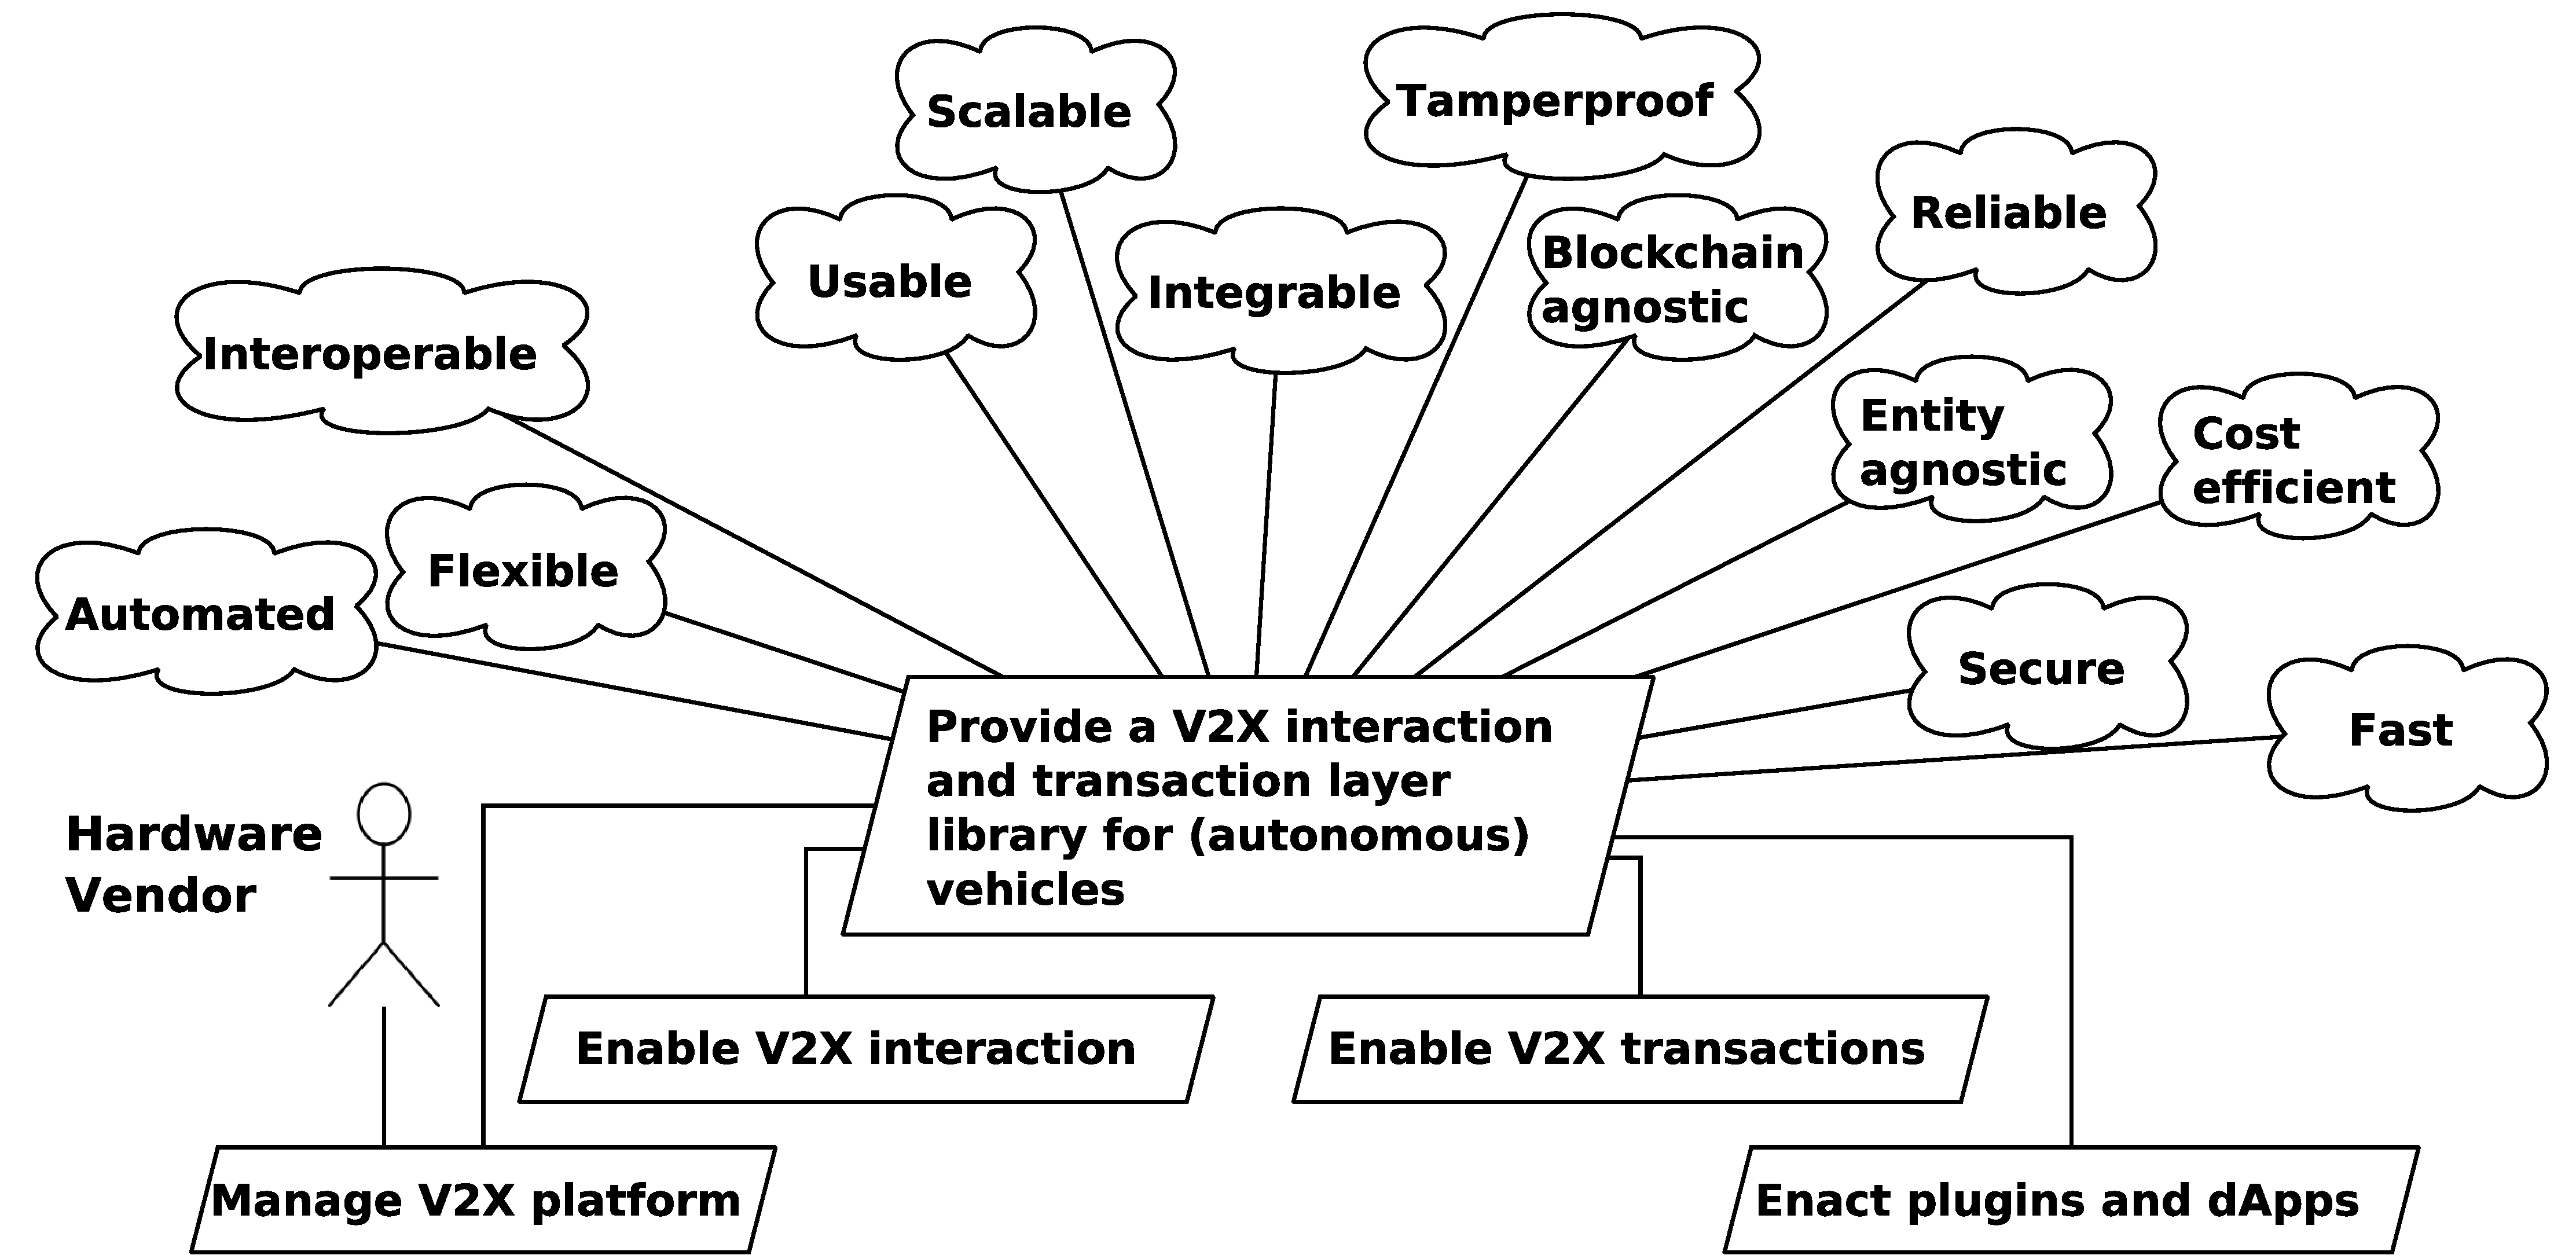
\includegraphics[scale=0.15]{Figures/aom/20180501_goal-model--top-level.pdf}
%					\caption{Chorus - Top-level goal model representation (Source: Based on \cite{leidingM2M}).}	
%					\label{fig:top-level-aom-goal-model}
%				\end{figure}
				
				\begin{figure}
					\centering
					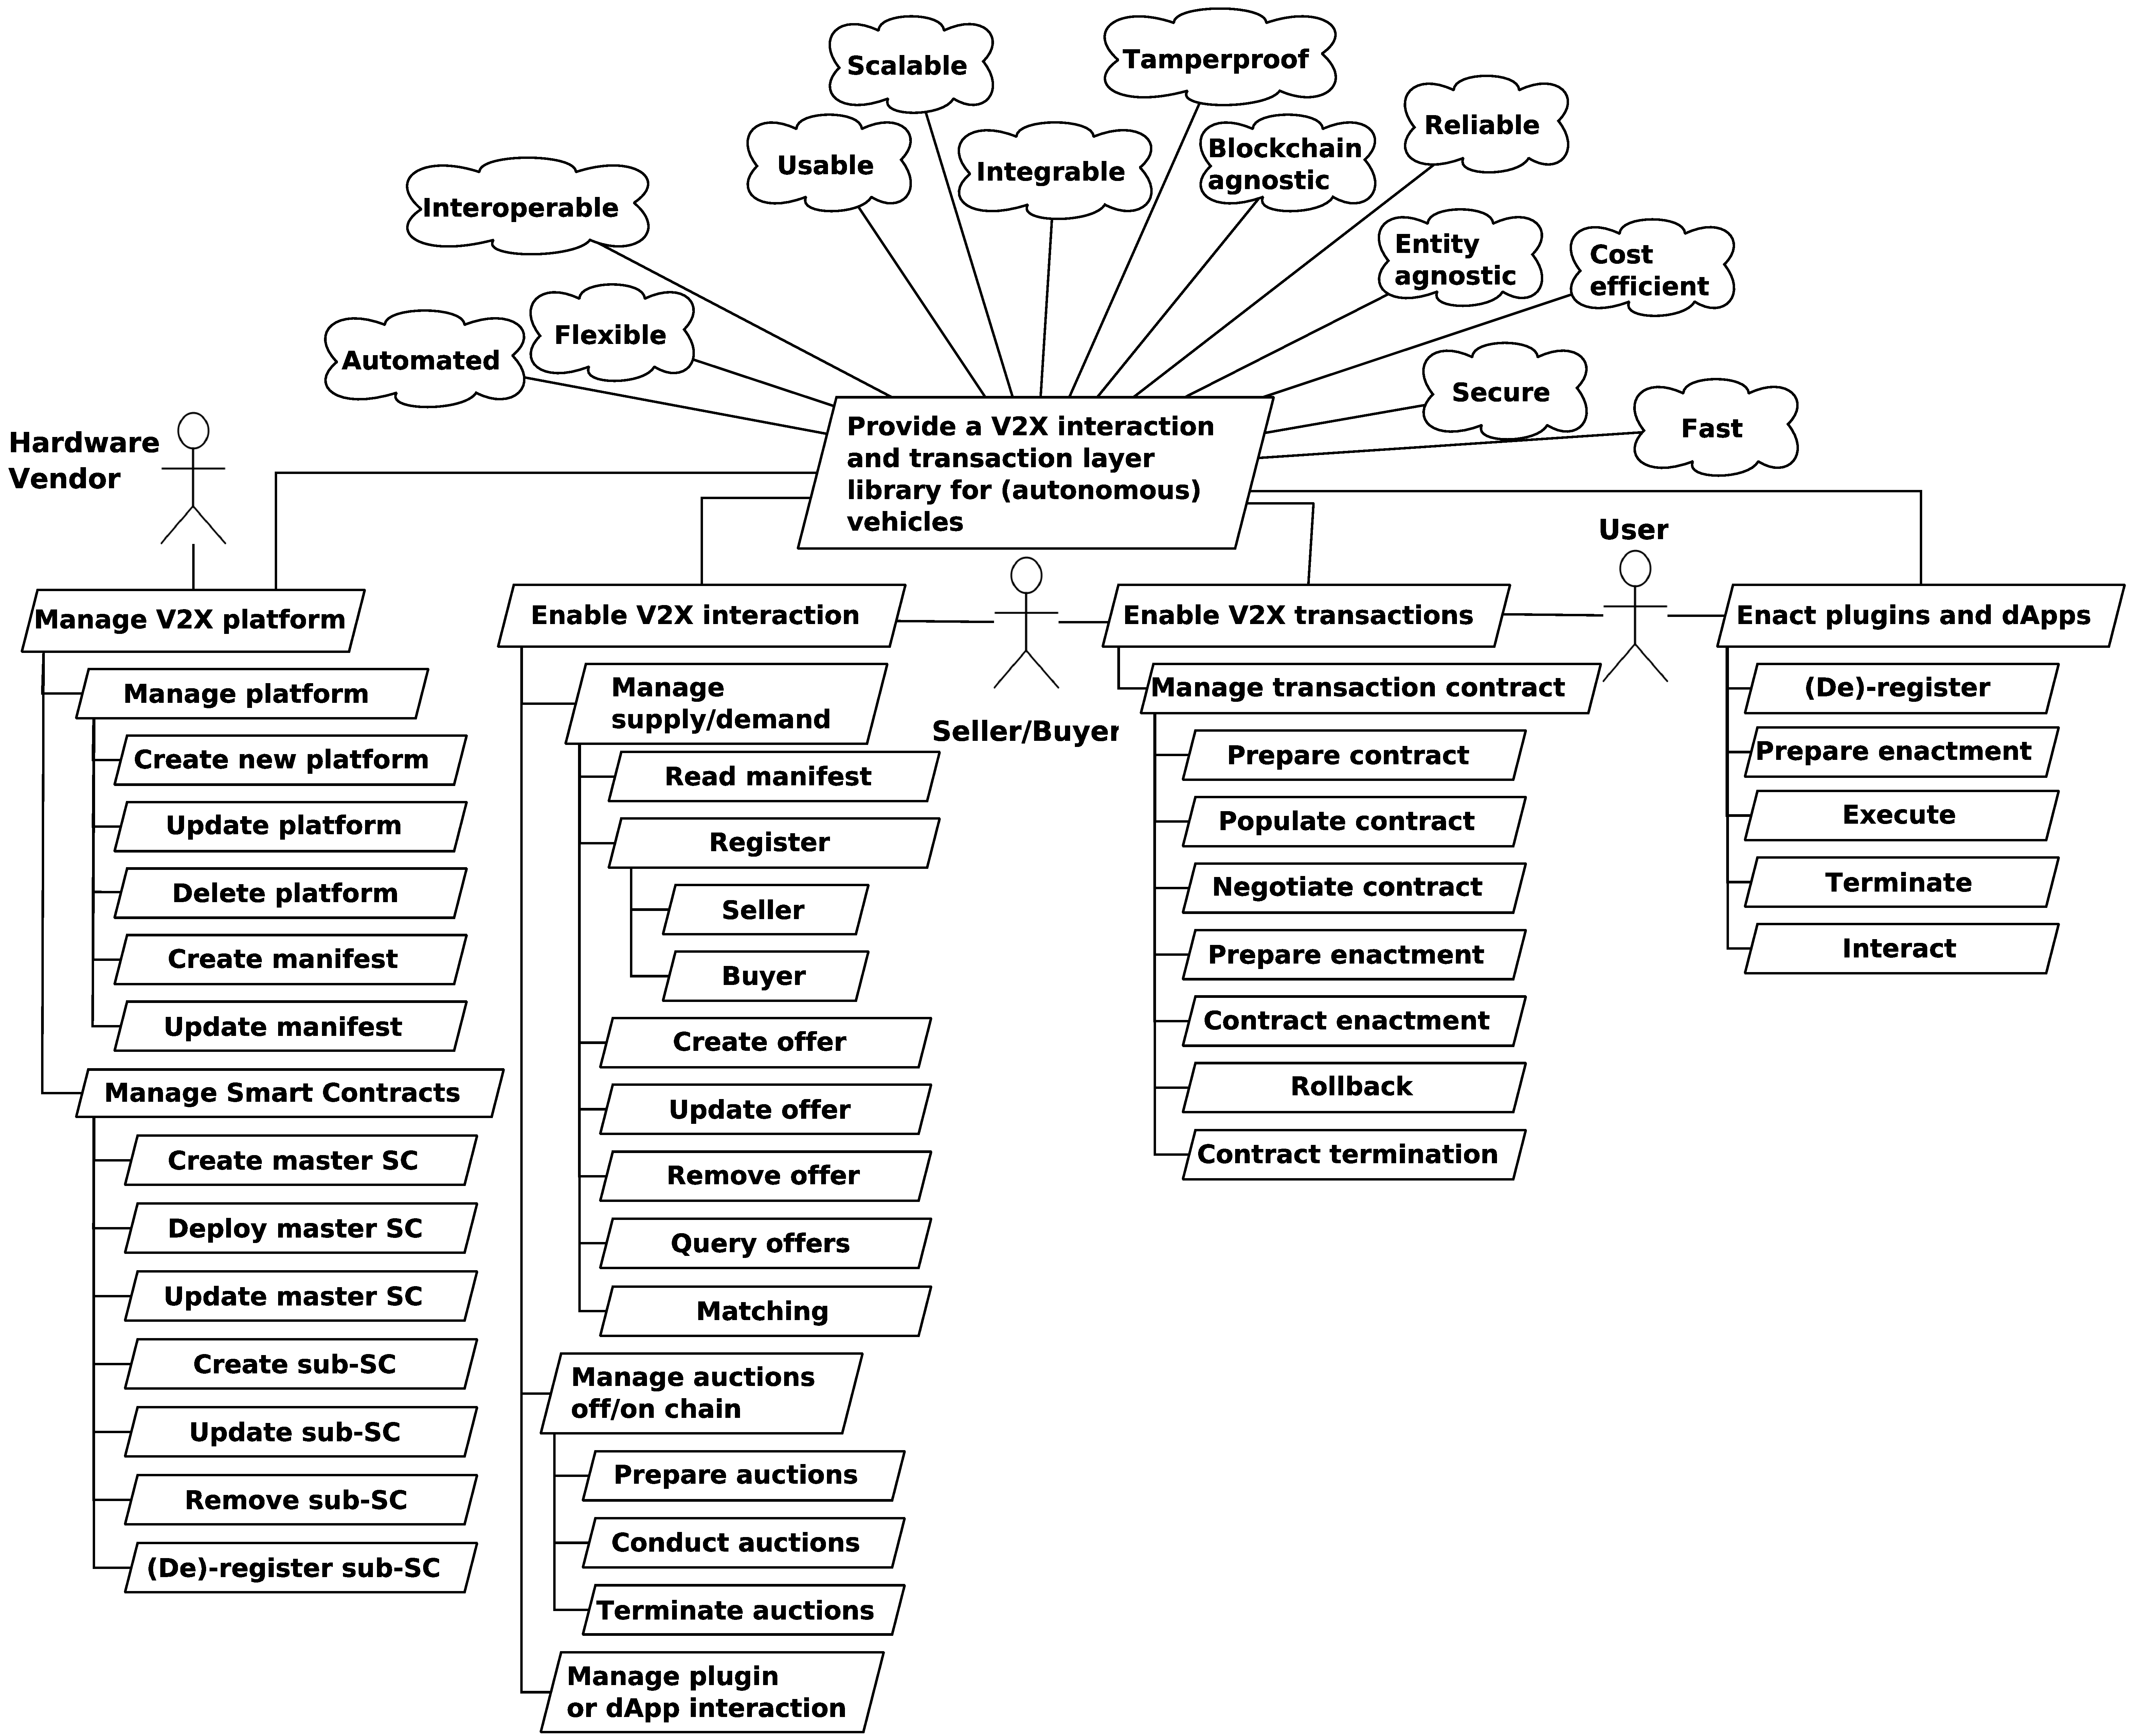
\includegraphics[scale=0.13]{Figures/aom/20180501_goal-model--complete.pdf}
					\caption{Chorus - Top-level goal model representation (Source: Based on \cite{leidingM2M}).}	
					\label{fig:top-level-aom-goal-model-extended}
				\end{figure}				

			\subsubsection{Non-Functional Requirements}
				\label{sss:quality-goals}
								
				Besides the four sub-goals of the top-level AOM goal model, we further identify thirteen quality goals of the main value proposition that are inherited to all refining sub-goals. A \textit{scalable} system design is necessary to provide Chorus services to a large quantity of users and customers. A further property that supports to achieve this scalability is the non-functional requirement \textit{automated}, that refers to a high degree of process automation eliminating the need for human interaction, e.g., tedious and repetitive tasks. \textit{Cost efficiency} is another important quality goal. \textit{Flexible} digital collaboration is a highly dynamic process that involves the enactment of diverse activities, the participation of diverse partners, and the exchange of diverse data \cite{norta2008exploring}. Thus, we must allow diverse collaboration scenarios and permit the inter-organizational harmonization of heterogeneous concepts and technologies between participating entities. Another key property of the system being easy to use (\textit{Usable}) for business collaboration. According to \cite{norta2014reference}, easy usability also includes the support of proper \textit{error avoidance} in order to ``anticipate and prevent common errors that occur during a collaboration configuration. Closely related is \textit{error handling}, to help with system support a user to recover from errors. \textit{Learnability} refers to how quickly users master using the system" \cite{norta2014reference}. 
				
				Moreover, we assign two additional quality goals that ensure a \textit{blockchain agnostic} as well as \textit{entity agnostic} design. Chorus should be neither limited to a specific blockchain nor vehicle hardware of a specific vendor. \textit{Interoperable} hardware and software design is another consequence of the previous quality goals as well as easy integration (\textit{Integrable}). It is crucial to interoperate at runtime with information systems supporting other business functions.
				
				Furthermore, a \textit{secure} service provision is also crucial in terms of operational security, e.g., protect user accounts and personal data from unauthorized access, secure data transfer within the system between entities or preventing data- and information leaks as well as preventing accidents. A \textit{reliable} enactment of all Chorus-based interactions and transaction facilitates the previous goals as well. Data communicated internally as well as externally has to protected against unauthorized tampering (\textit{tamperproof}) in order to protect business collaborations, but also ensure the safety of participating entities. Finally, since cars and similar vehicles move much faster than humans, a \textit{fast} service provision is essential for most tasks.
			
			%% ----------------------------------------------------------------
			%% ----------------------------------------------------------------	
					
%			\subsubsection{Refined AOM Goal Model}				
%				\label{sss:refined-goal-model}			
%
%				\begin{figure}[H]
%					\centering
%					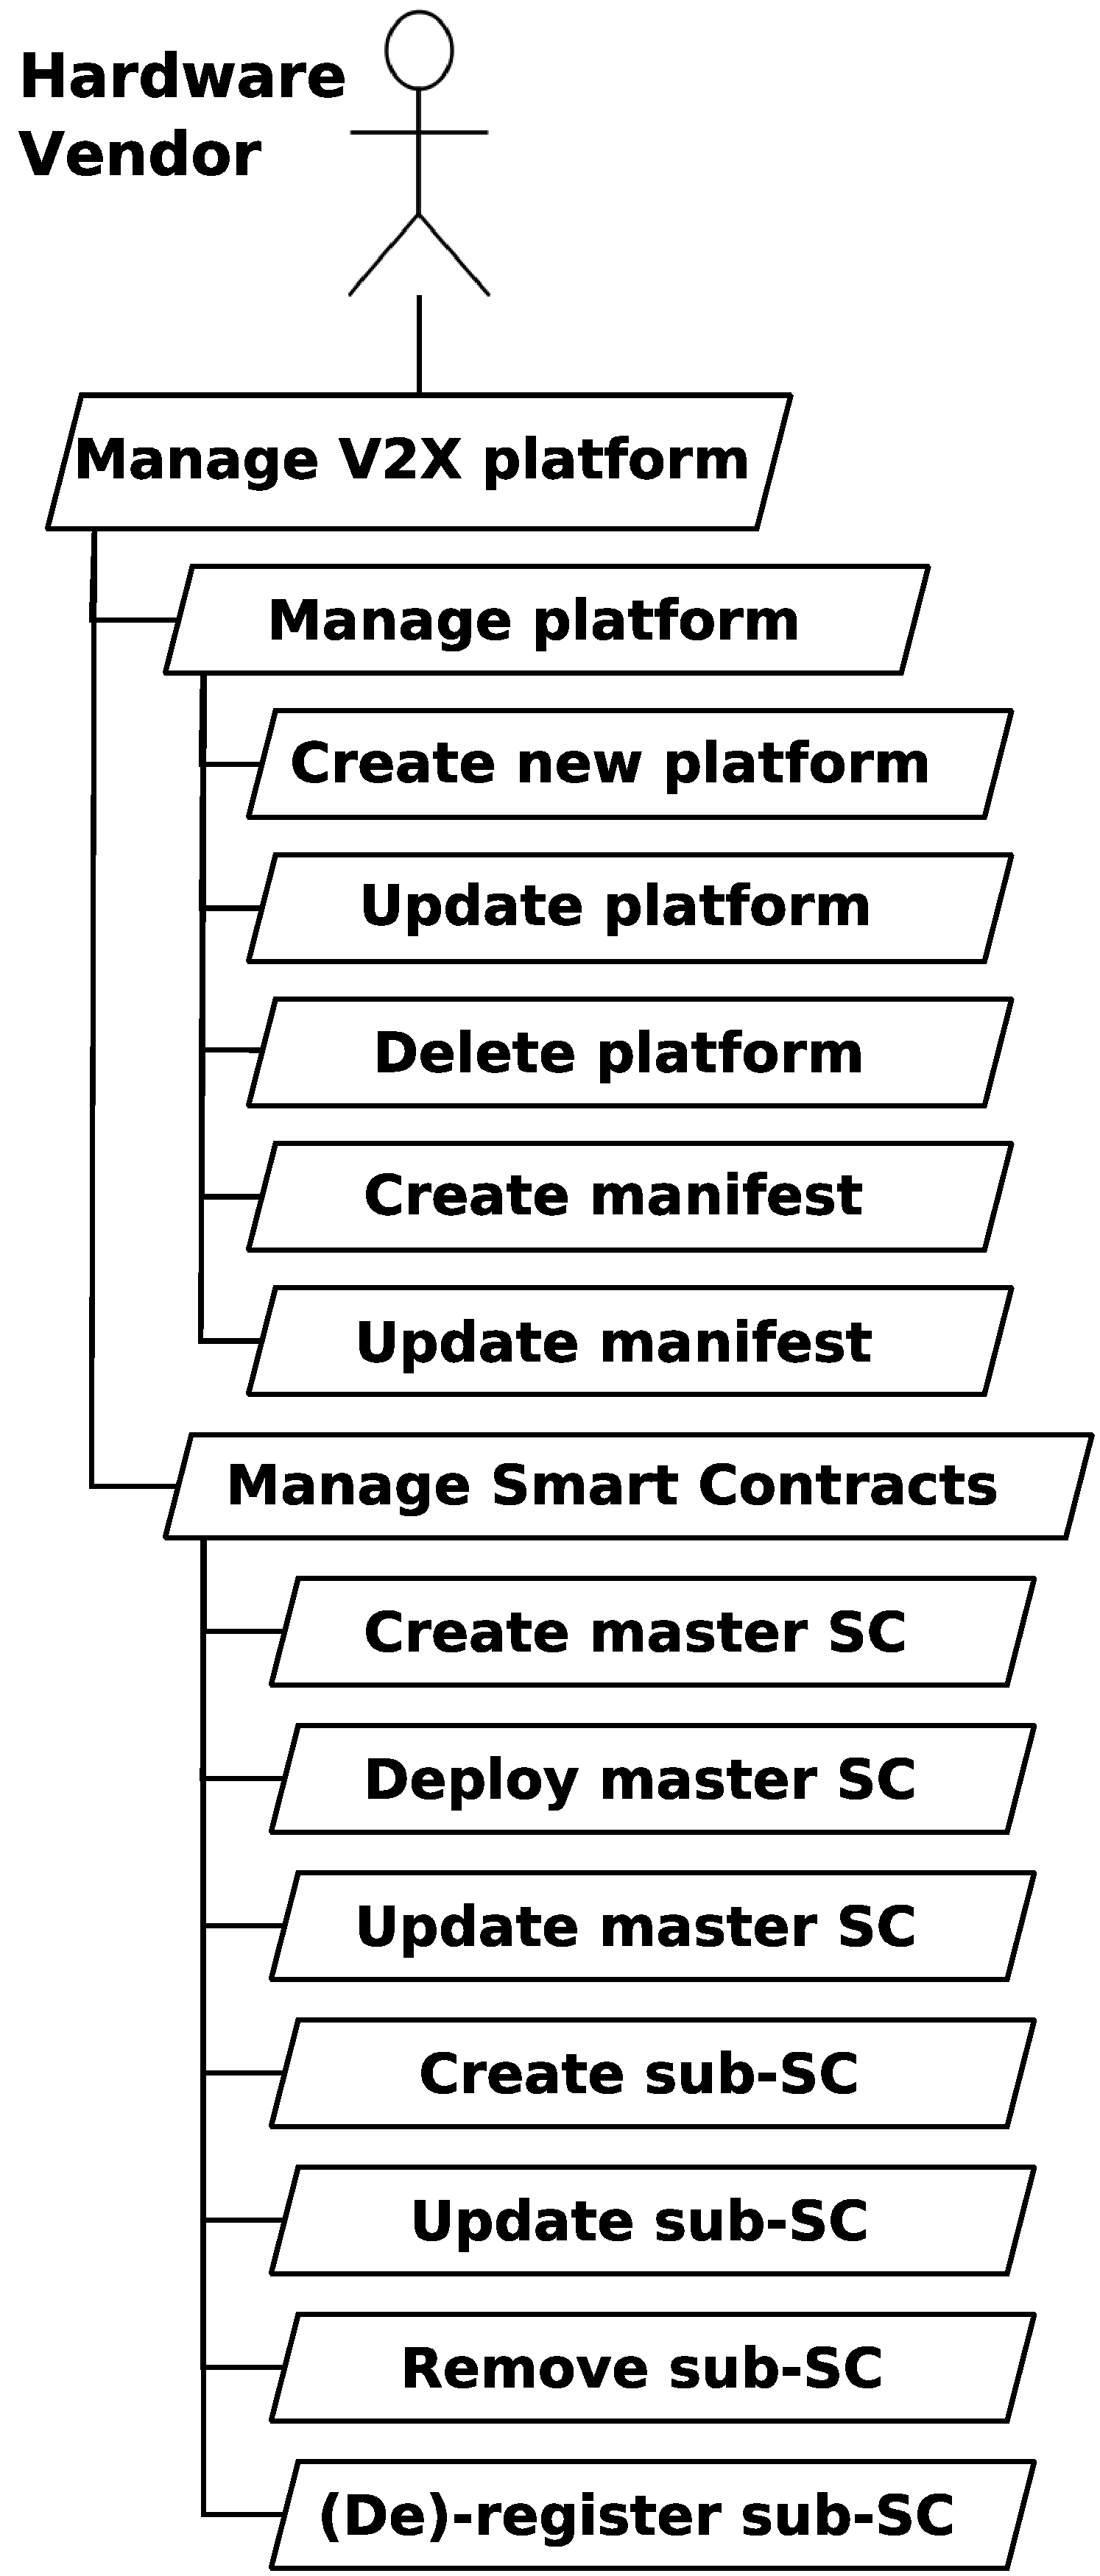
\includegraphics[scale=0.175]{Figures/aom/20180501_goal-model--refined-1.pdf}
%					\caption{Chorus - Goal model refinement \textit{Manage V2X platform} (Source: Based on \cite{leidingM2M}).}	
%					\label{fig:refined-aom-goal-model-1}
%				\end{figure}
%				
%				\begin{figure}[H]
%					\centering
%					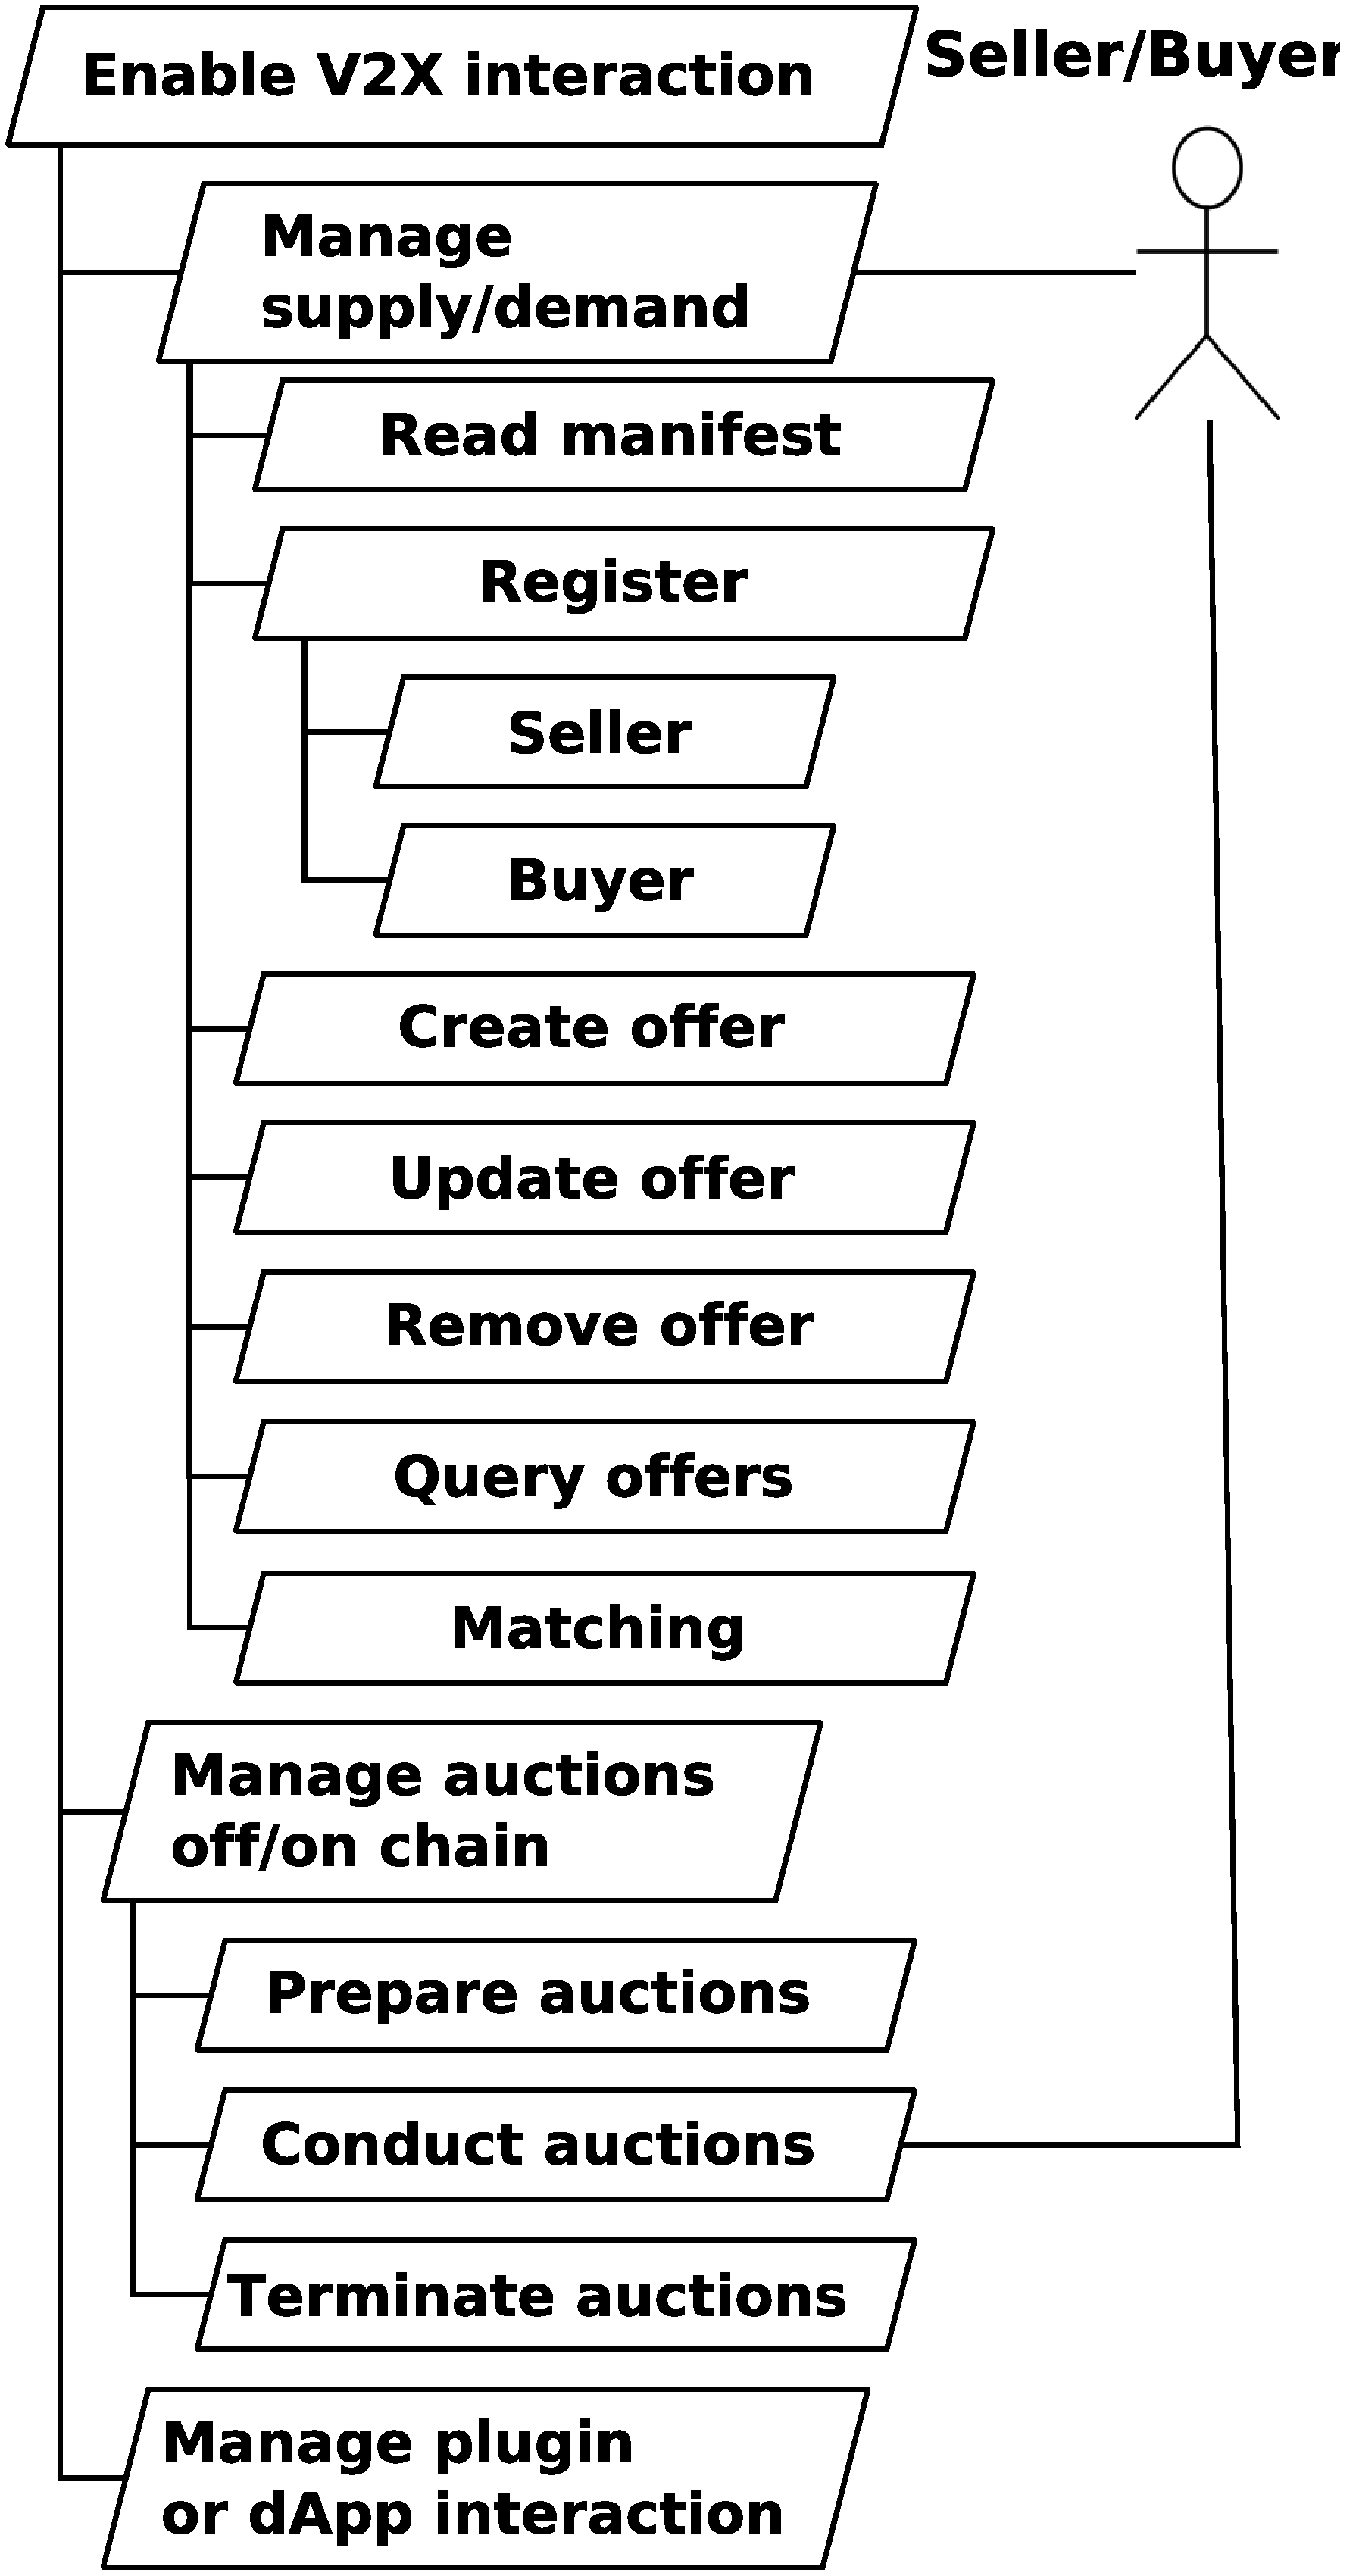
\includegraphics[scale=0.175]{Figures/aom/20180501_goal-model--refined-2.pdf}
%					\caption{Chorus - Goal model refinement \textit{Enable V2X interaction} (Source: Based on \cite{leidingM2M}).}	
%					\label{fig:refined-aom-goal-model-2}
%				\end{figure}				
%	
%				\begin{figure}[H]
%					\centering
%					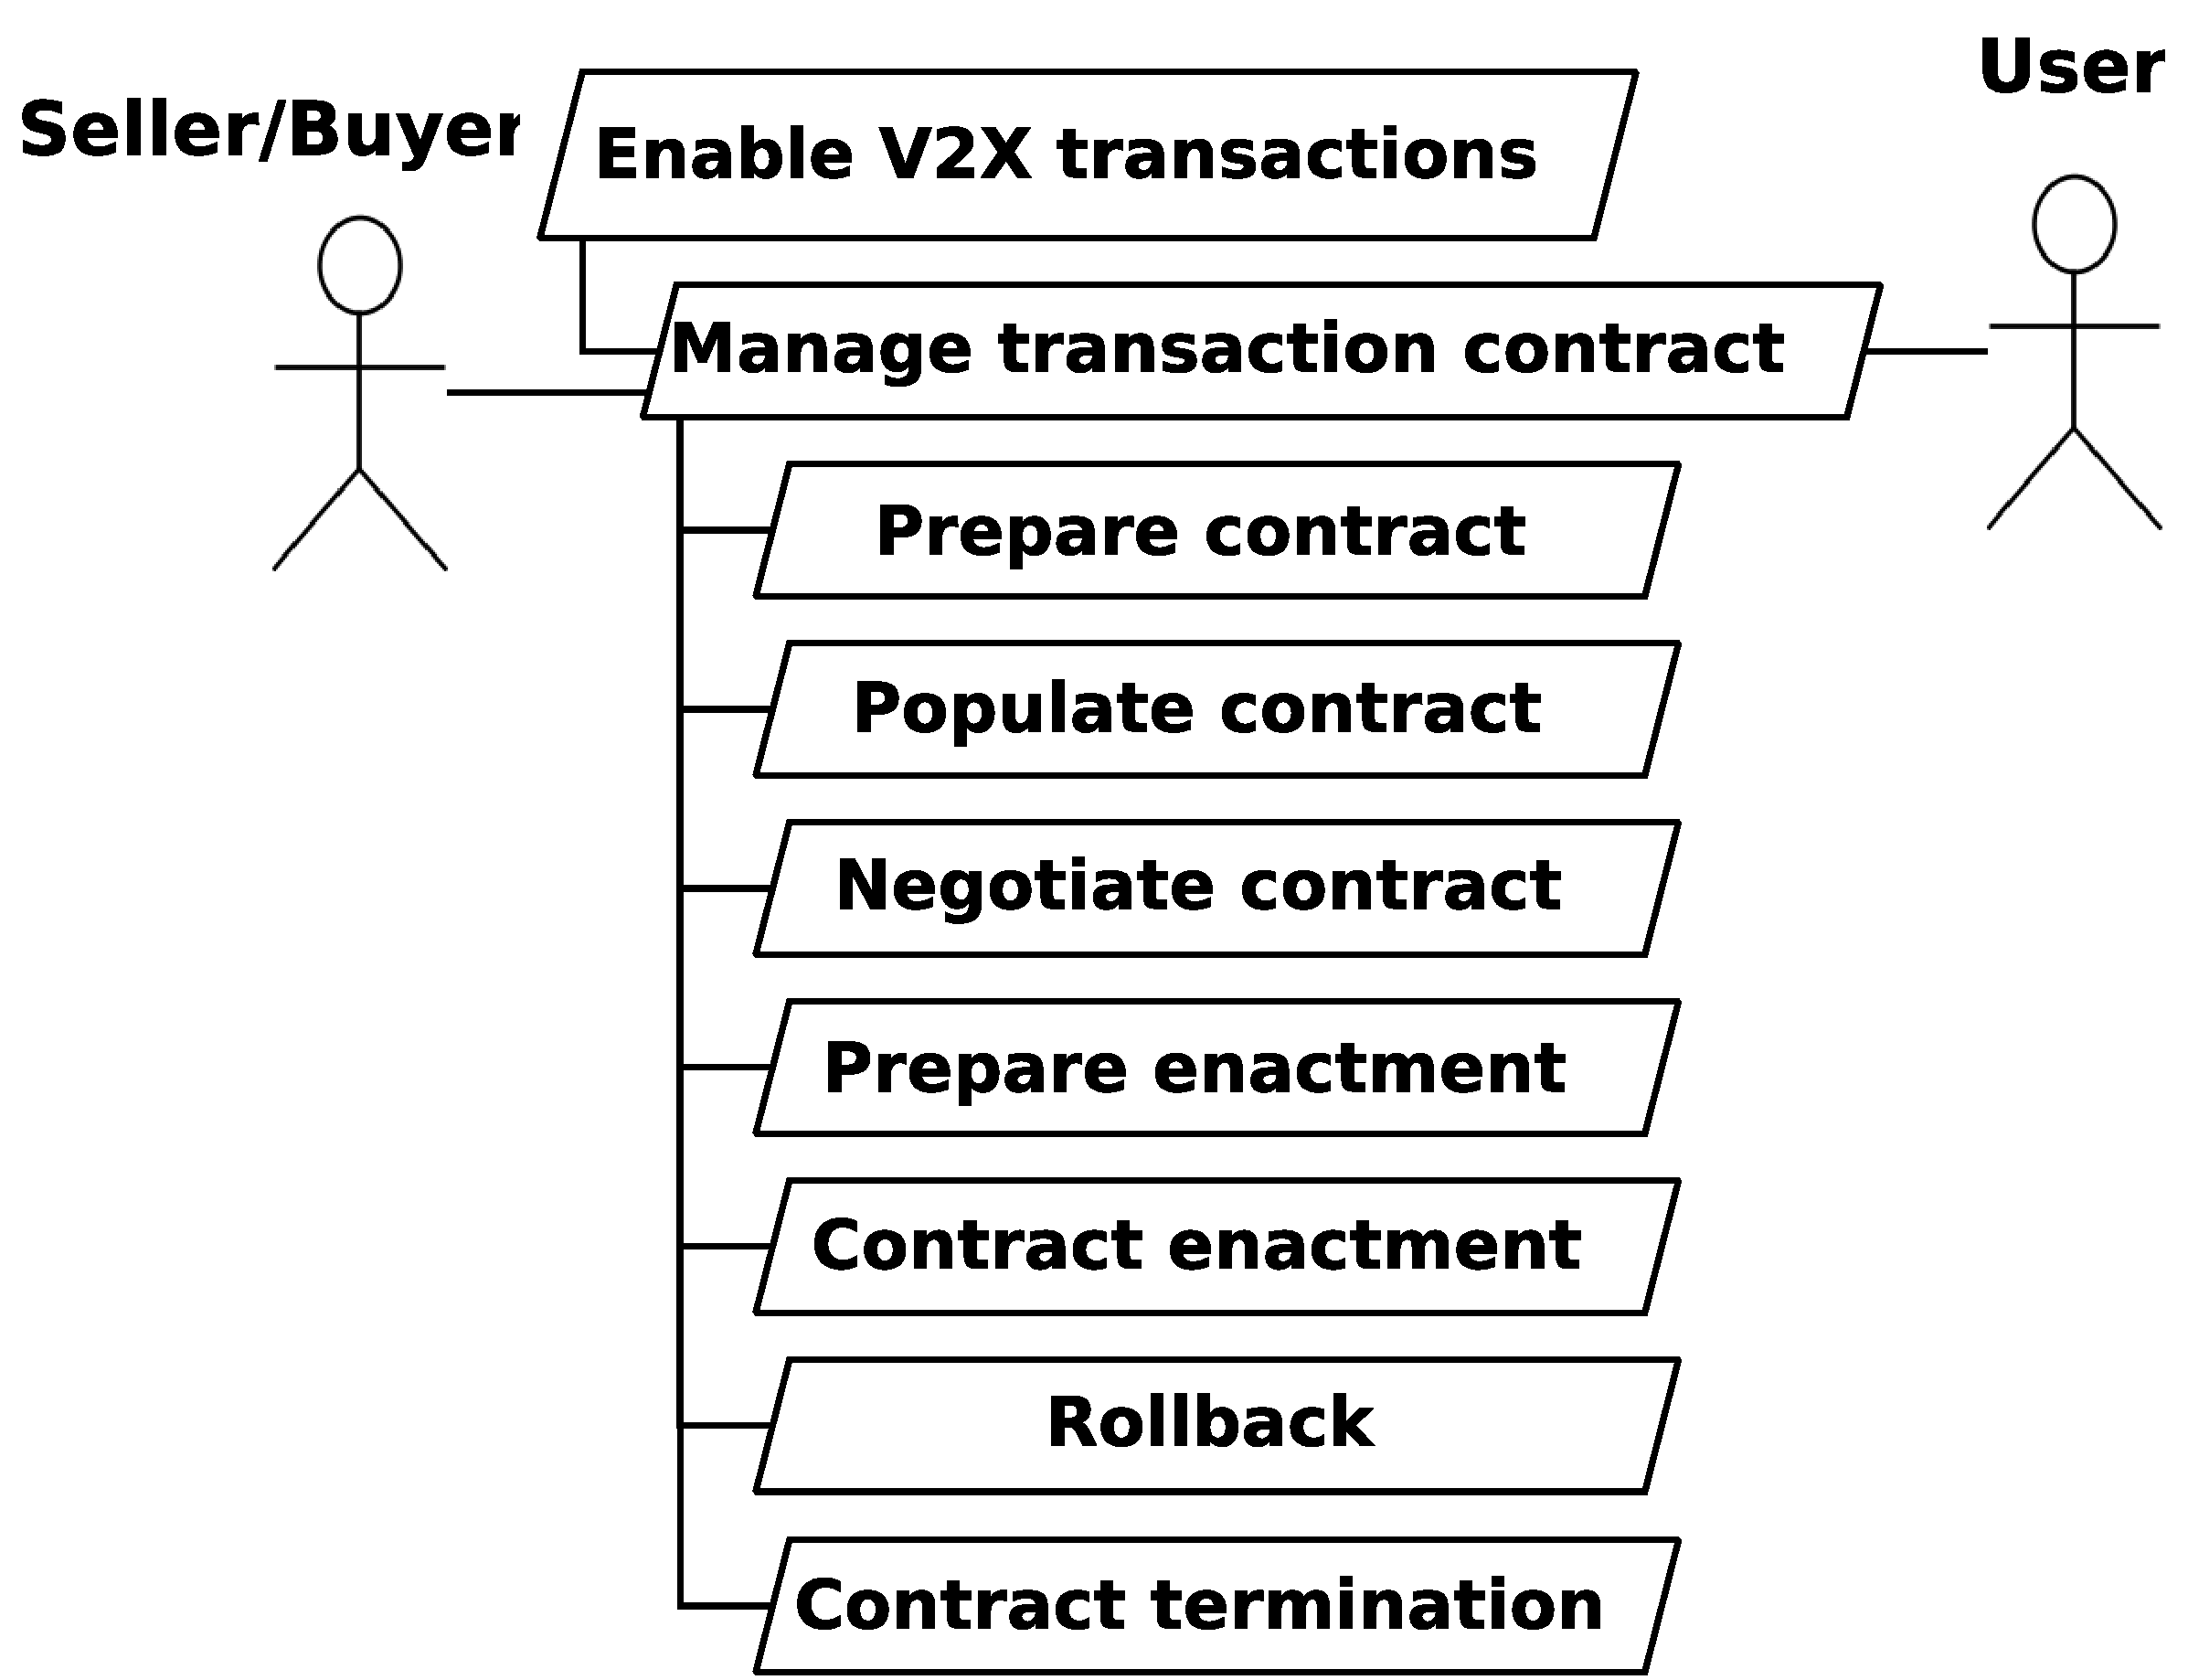
\includegraphics[scale=0.175]{Figures/aom/20180501_goal-model--refined-3.pdf}
%					\caption{Chorus - Goal model refinement \textit{Enable V2X transaction}  (Source: Based on \cite{leidingM2M}).}	
%					\label{fig:refined-aom-goal-model-3}
%				\end{figure}
%				
%				\begin{figure}[H]
%					\centering
%					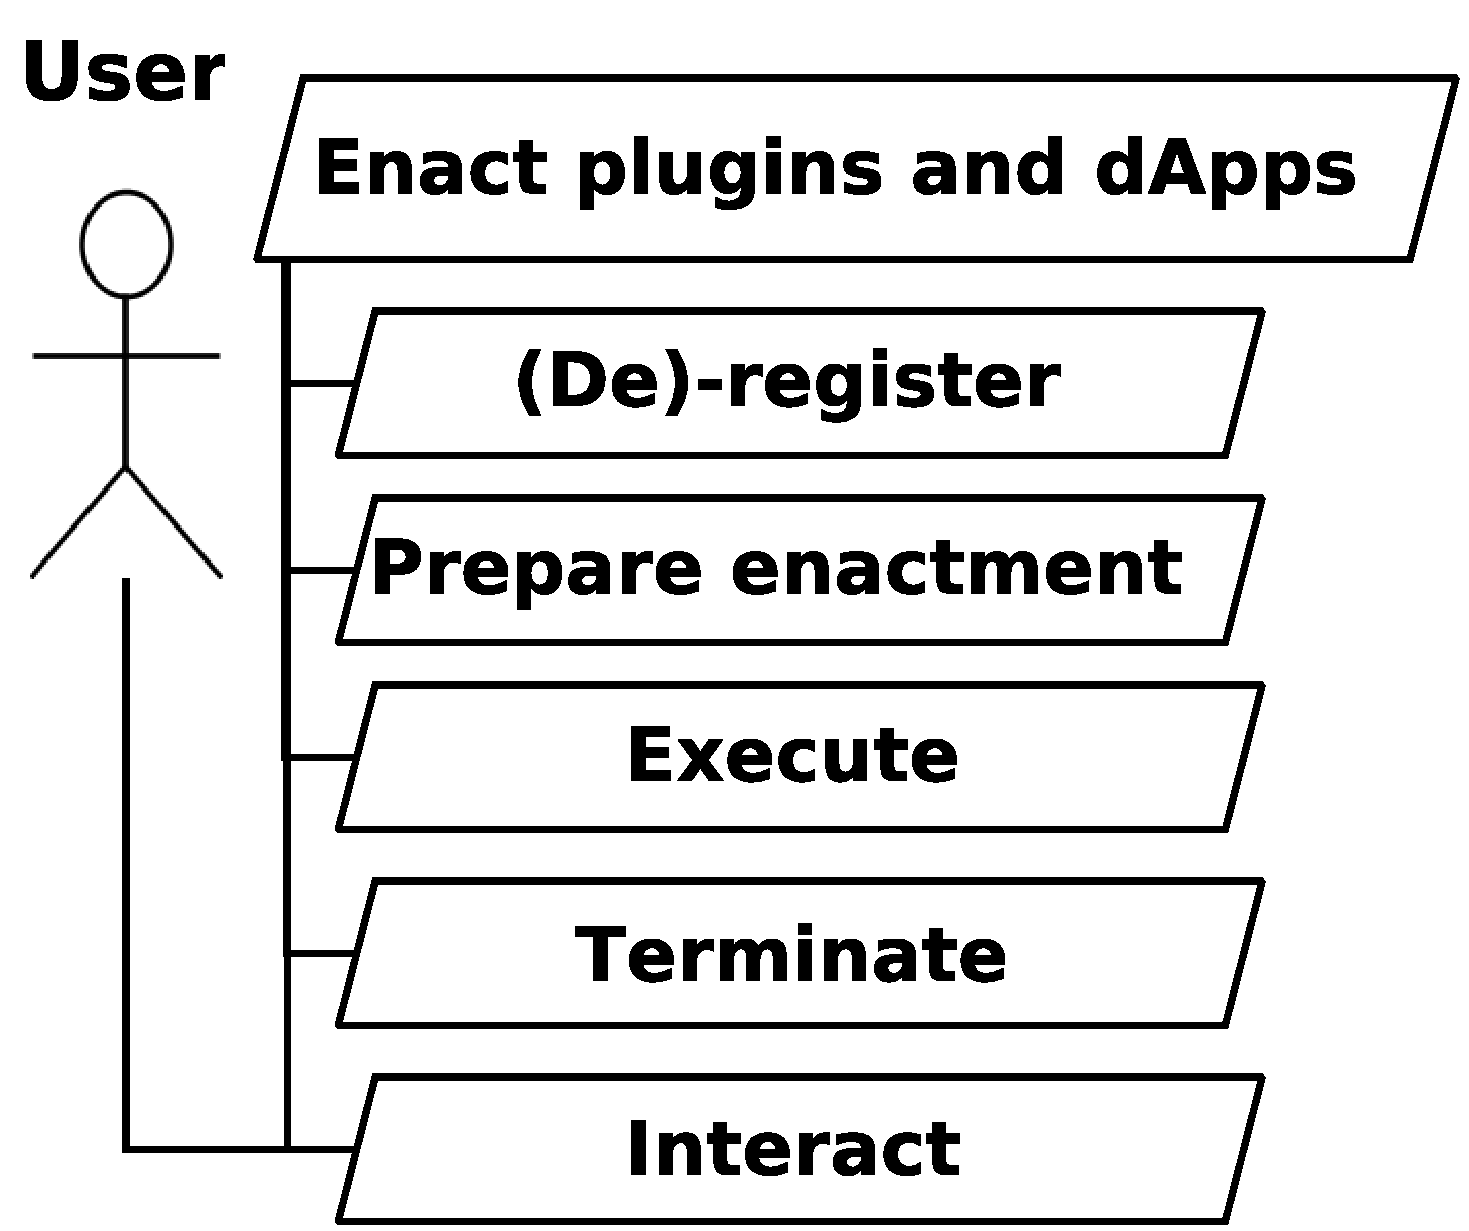
\includegraphics[scale=0.175]{Figures/aom/20180501_goal-model--refined-4.pdf}
%					\caption{Chorus - Goal model refinement \textit{Plugin and dApp enactment}.}	
%					\label{fig:refined-aom-goal-model-4}
%				\end{figure}


			The presented goal model is used in the following Section \ref{ss:component-diagrams} to derive our system architecture. We do not list all details of the further refined AOM goal model in this whitepaper due to space constraints and in order to focus on the most relevant system components and features.
									
			%% ----------------------------------------------------------------
			%% ----------------------------------------------------------------				

		%% ----------------------------------------------------------------
		%% ----------------------------------------------------------------	
		
		\subsection{System Architecture}
			\label{ss:component-diagrams}

			The abstract system- and business architecture is derived from the functional- and non-function requirements of the AOM goal model presented earlier. The services are powered by a service-oriented architecture (SOA) that is comprised of different designated components. Each of these components is self-contained, well-defined components and provides a specific set of services \cite{erl2005service}\cite{perrey2003service}. Dedicated services and components may also consist of other underlying sub-services \cite{rosen2012applied}. 
			
			In the following, a technology-agnostic UML-component-diagram representation is used to illustrate the system architecture \cite{booch1996unified}\cite{specification2007omg}. The UML notation elements used to model the architecture are presented in Figure \ref{fig:uml-component-diagram-overview}. In UML, components are represented as rectangular boxes and labeled either with the keyword \textit{component}, or with the component icon in the right-hand upper corner. A component may consists of further sub-components and is implemented by one, or more classes, or objects. Moreover, components are reusable and communicate via two types of interfaces as illustrated in Figure \ref{fig:uml-component-diagram-overview}. Small squares depict ports that are attached to the border of components and expose required and provided interfaces. Ports may also specify inputs and outputs as they operate uni-, or bi-directionally \cite{booch1996unified}\cite{specification2007omg}. Once more, sticky men are used to depict entities and their interactions with the system. 
			
			\begin{figure}[H]
				\centering
				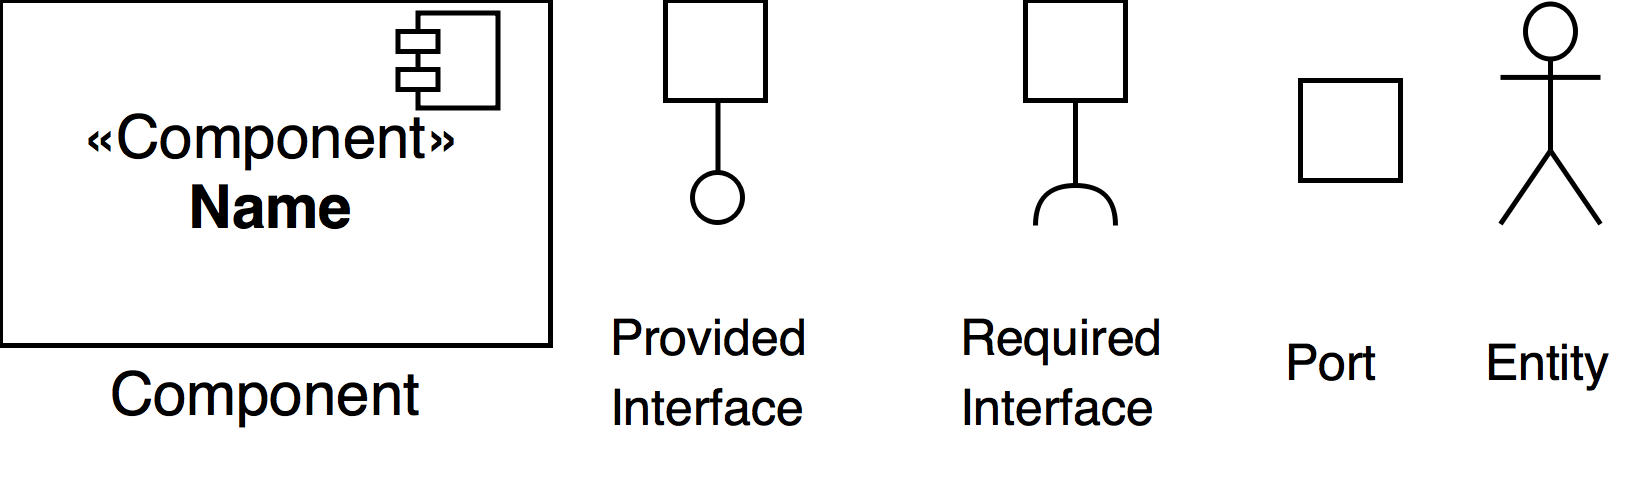
\includegraphics[scale=0.12]{Figures/UML-notation-elements.png}
				\caption{UML-component diagram notation elements.}	
				\label{fig:uml-component-diagram-overview}
			\end{figure}	
			
			The remainder of this section first introduces an abstract high-level overview of the system architecture and components. Afterwards, further illustration present selected sub-components of our architecture.


			%% ----------------------------------------------------------------
			%% ----------------------------------------------------------------	

			\subsubsection{High-Level Architecture}
				\label{sss:high-level-architecture}
				
				The highest architecture abstraction level of our system is depicted in Figure~\ref{fig:high-level-architecture}. The representation is divided into two distinct packages, e.g, the Blockchain package and the Vehicle-System package. In UML, packages are used “to group elements, and provide a namespace for the grouped elements”  \cite{specification2007omg}. In the context of this architecture illustration, packages are used to provide a separation of concerns between the blockchain part and the vehicle related system components, as well as the Chorus mobile smartphone application. The vehicle-system package consists of three main components, e.g., the Chorus firmware, the vehicles manufacturer OS and the component managing the underlying hardware of the vehicle, and several smaller components that will be detailed in Section~\ref{sss:architecture-refinements}.
				\begin{figure}[H]
					\centering
					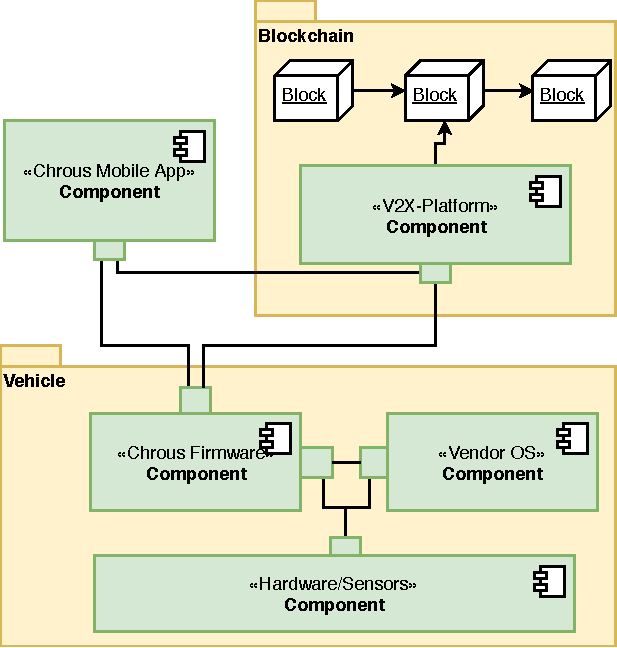
\includegraphics[scale=0.75]{Figures/longterm-architecture/20180507_high-level-architecture.pdf}
					\caption{High-level architecture of the Chorus V2X system.}	
					\label{fig:high-level-architecture}
				\end{figure}					
				The blockchain package comprises the V2X platform itself and the blockchain utilized by Chorus to enable our services. The following Section~\ref{sss:architecture-refinements} explains each of the units illustrated in Figure~\ref{fig:high-level-architecture} in detail.
			
			%% ----------------------------------------------------------------
			%% ----------------------------------------------------------------	
			

			\subsubsection{Selected Architecture Refinements}
				\label{sss:architecture-refinements}
			
				The following illustration represent visualization of the Chorus longterm architecture. We simplified certain aspects due to space constraints and to reduce technical complexity.First, Figure~\ref{fig:system-architecture--app} shows the different components of the \textit{Chorus Mobile App} component, e.g., the user interface (UI) component, the settings/preferences component, the wallet component, the communication component and the chorus application management component. The UI-component is the gatekeeper for the user and used to control all functionalities from the user side and also to interact with the system. The user can set preferences and change settings, visualize wallet balances, activate plug-ins or Chorus applications (we only listed two as an example) such as the ``Good-driving-behavior-plug-in. The wallet component holds the users public and private key pair that represent the wallet address. The user can transfer tokens from and to his/her wallet to use Chorus-compatible services or applications. The user's smartphone is connected to the vehicle component and utilizes the communication component to communicate with the vehicle component as well as the V2X platform. Besides these functional components, Figure~\ref{fig:system-architecture--app} also contains the Android OS component and the underlying hardware (GPS, Wifi, USB, bluetooth, etc.) of the smartphone for easier visualization purposes.

				\begin{figure}
					\centering
					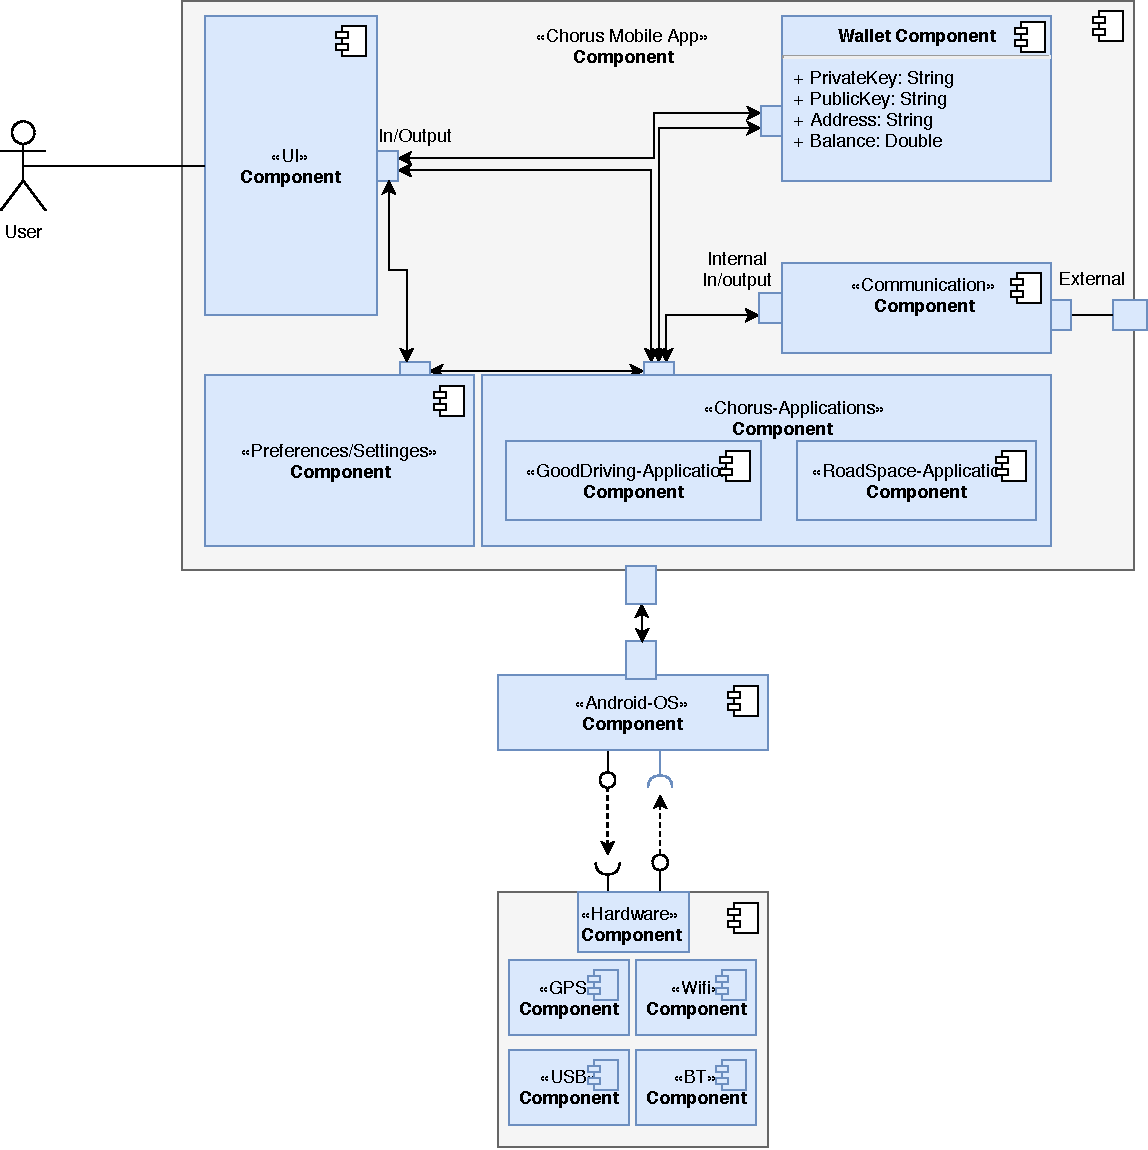
\includegraphics[scale=0.65]{Figures/longterm-architecture/20180507_Refined-sys-architecture--mobile-app.pdf}
					\caption{Refined illustration of the \textit{Chorus Mobile App} component.}	
					\label{fig:system-architecture--app}
				\end{figure}
				Next, Figure~\ref{fig:system-architecture--vehicle} presents a more detailed view of the \textit{vehicle} sub-system. In the beginning, this sub-system is located in a dedicated box that is connected to the user's smartphone via bluetooth or Wifi, the V2X platform via the Internet, to other vehicles via the WAVE protocol stack \cite{li2010overview}\cite{uzcategui2009wave} as  well as the vehicle via OBDII - hence we have a dedicated communication component on the left as well as the right for each of these two functionalities. The OBDII interface is used to query information from the car such as speed, steering, breaks and many more. The information are used by Chorus applications and plug-ins to provide their services. The logic of the Chorus applications mostly resides in the Chorus plug-in component of Figure~\ref{fig:system-architecture--vehicle} while the Chorus application component in Figure~\ref{fig:system-architecture--app} is mostly used to control the applications and enable them on the dedicated Chorus box. The Chorus component in Figure~\ref{fig:system-architecture--vehicle} also contains the Chorus firmware as well as the blockchain client(s). 
			
				Due to the speed of moving cars, most of the time on-chain auctions are not an option and instead auctions or negotiation on a local level between nearby vehicles are necessary. The auction components contains all functionalities to do that as well as settings that control the auction preferences of the vehicles. More details on the actual workflow of the off/on-chain auctions are available in Section~\ref{ss:auchtion-algorithm}.
							
				In the future, when most people do not own cars themselves any more, users can transfer tokens to the vehicles wallet to pay for taxi services and the vehicle uses these earnings to pay for electricity or maintenance. Hence, the vehicle also has a separate wallet for this purpose.
				
				Similar to the previous Figure~\ref{fig:system-architecture--app}, at the bottom we list hardware-focused components such as the different sensors that may reside in the vehicle or the Chorus box, different hardware connectors and the tamperproof device (TPD) that controls the car's identity, authenticates exchanged messages and data packets and so on.
				
				\begin{figure}
					\centering
					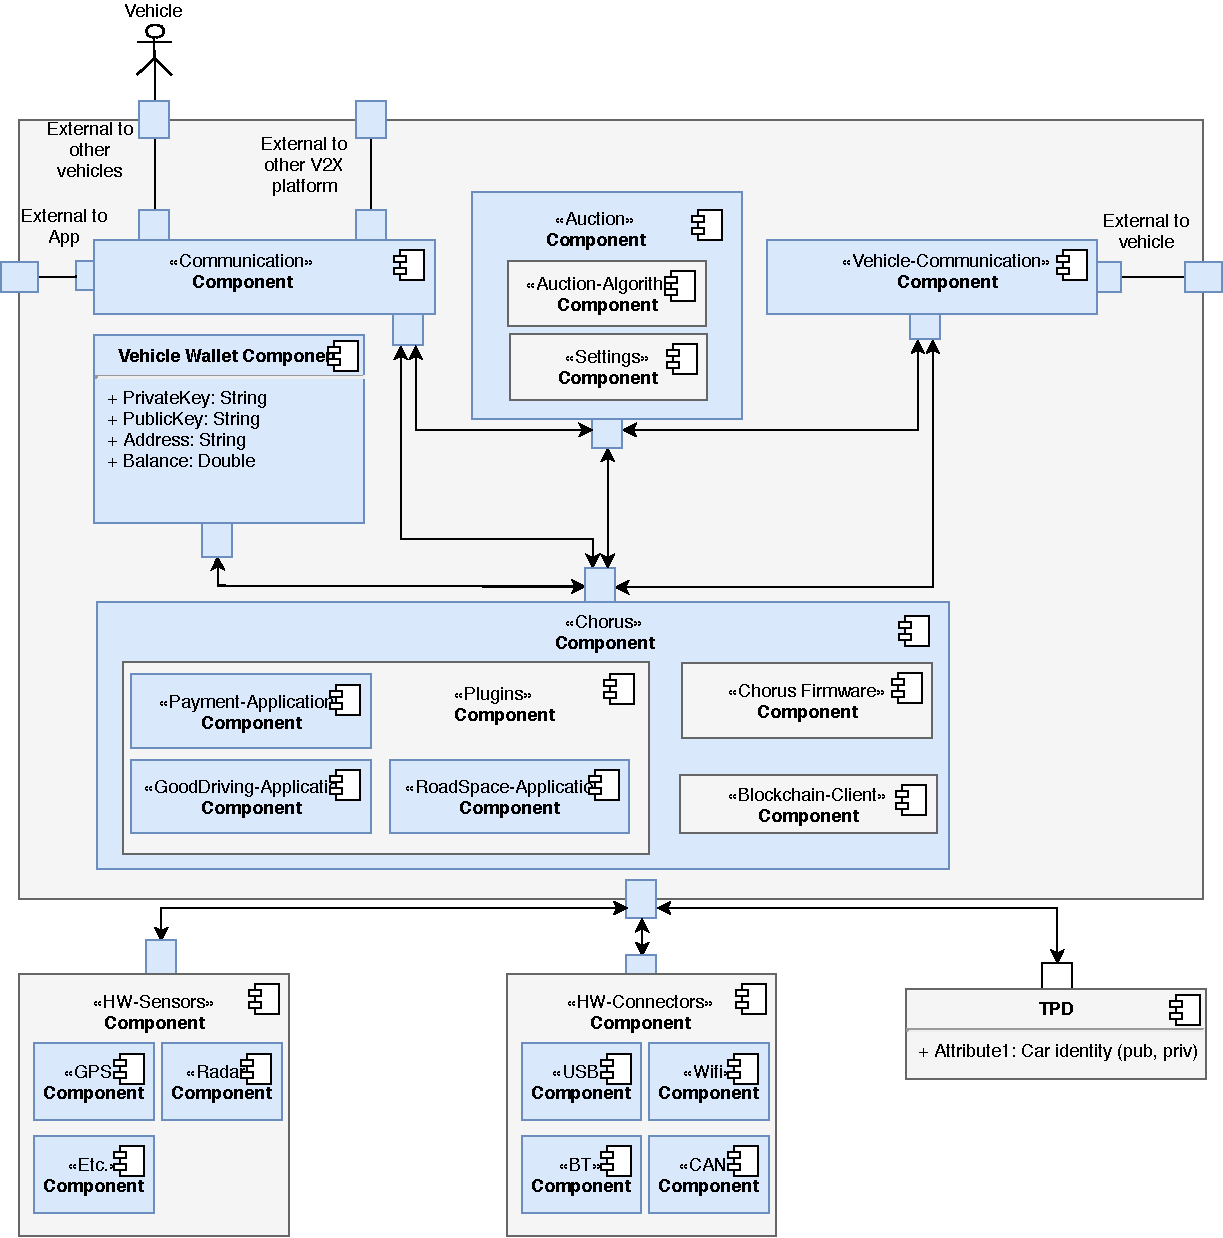
\includegraphics[scale=0.65]{Figures/longterm-architecture/20180507_Refined-sys-architecture--vehicle.pdf}
					\caption{Refined illustration of the \textit{Vehicle} sub-system.}	
					\label{fig:system-architecture--vehicle}
				\end{figure}
				
				Finally, Figure~\ref{fig:system-architecture--platform} presents a more detailed view of the \textit{V2X platform} sub-system. As before for all the other sub-system, the V2X platform also contains a communication component managing the communication between the platform and the blockchain and vehicles. In addition, the respective platform management entity (Chorus or a vehicle manufacturer that is running their own Chorus compatible platform) has access to an administration interface. The administrator uses this interface to maintain the platform and the corresponding smart contracts as well as the user management and much more. Similar to the auction component in the previous Figure~\ref{fig:system-architecture--vehicle}, the V2X platform has a component that takes care of on-chain auctions using the same auction algorithms. Auctions may result based on the supply and demand management that is conducted in the corresponding component. Finally, similar to the application/plug-in components in the mobile application and the vehicle, we also have a pendant of these component in the V2X platform. Here, the component is mainly used for application/plug-in related interaction and transaction enactment.
				
				\begin{figure}
					\centering
					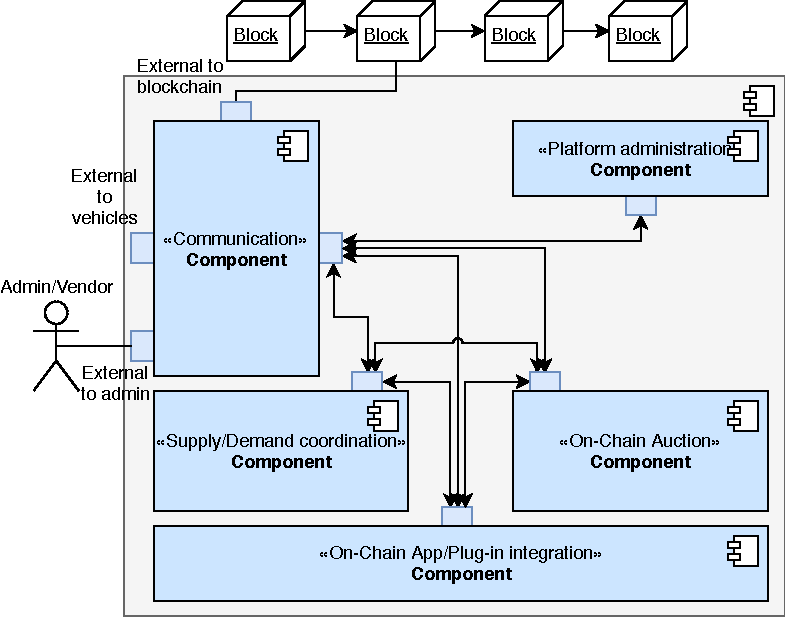
\includegraphics[scale=0.75]{Figures/longterm-architecture/20180507_Refined-sys-architecture--V2X.pdf}
					\caption{Refined illustration of the \textit{V2X-Platform} sub-system.}	
					\label{fig:system-architecture--platform}
				\end{figure}						

%	Notes
%		- foam
%		- infura
%		- a general technology section			
%		Pitch Deck Problems for Will:
%		
%		1.) Fast moving vehicles vs. slow blockchains
%		Figure out a what actions/functionalities/process to put on/off-chain 
%		
%		2.) Amount and size of transmitted data
%		Even if each car transmits only 10MB of data per hour, this gets ridiculous even if we only have 1 million vehicles that use our system
%		
%		3.) Efficient auction/trading algorithm
%		
%		4.) Localization and organization of vehicle positions
%		How do I figure out if the car that is sending me messages is behind me, in front of me or on my righ/left-hand side?			
%		



		%% ----------------------------------------------------------------
		%% ----------------------------------------------------------------	
		
%		\subsection{Library / API}
%			\label{ss:library-api}				
%			\textbf{Work-In-Progress}
%			
		%% ----------------------------------------------------------------
		%% ----------------------------------------------------------------	

		Next, in Section~\ref{s:section-5} we present the system-engagement processes of the the Chorus V2X system using and outline the interaction workflow of the on/off-chain auction algorithms.


	%% ----------------------------------------------------------------
	%% ----------------------------------------------------------------
	
	\section{System Engagement Processes}
		\label{s:section-5}	
	
		%% RQ-3: What are the system-engagement processes for the stakeholders?
	
		The Chorus transaction layer library automates and simplifies VANET-based V2X service provision on several levels. A core element of many of the Chorus use cases is smart contract-based negotiation and contract enactment between entities that are the result of collaborating tasks and subprocesses. For example, as described in Section~\ref{s:section-2} two vehicles conduct a road-space negotiation auction that results either in a change of positions or is aborted. This process potentially also involves payment processing, further local as well as global communication and local match-making between vehicles. On an abstract level, most of the use cases presented earlier in this paper follow at some point a similar procedure on smart-contract level. Same applies for scenarios that involve a price negotiation or auction. In the following, we introduce these two abstract processes in more detail
		The processes are represented using Business Process Model and Notation (BPMN) \cite{model2011notation} and UML sequence diagrams \cite{msequenceDiagrams}.
		
		Consequently, Section~\ref{ss:smart-contract-lifecycle-management} details the BPMN representation of the generalized contract negotiation lifecycle, followed by Section~\ref{ss:auchtion-algorithm} that details the different auction mechanisms of our platform. Finally, Section~\ref{ss:token-economics} covers the Chorus token value proposition.



		%% ----------------------------------------------------------------
		%% ----------------------------------------------------------------	
		
		\subsection{Smart Contract Negotiation Lifecycle Management}
			\label{ss:smart-contract-lifecycle-management}
			
			The abstract smart contract negotiation lifecycle, as illustrated in Figure~\ref{fig:smart-contract-lifecycle-management}, is divided into the following stages: a) preparatory, b) negotiation, c) contract execution d) rollback and e) a contract expiry stage. During the preparatory stage, information regarding the involved entities, such as identifiers and wallet addresses are incorporated into the contract. In addition, the conditions of the requested contract are formally defined by specifying, e.g, the content and target of the contract. Following, the example of the cab service for a human, this might include the start location, final destination, price, and so on. The conditions of the requested cab-ride mainly depend on information such as the travel distance and fuel/energy consumption of the vehicle. In case the vehicle and the user agree on the negotiated conditions, both parties sign the contract and express their approval - if no agreement is reached, a contract rollback is triggered. After signing the agreement, the contract execution phase is triggered and the the vehicle picks up the user. 

			\begin{figure}[H]
				\centering
				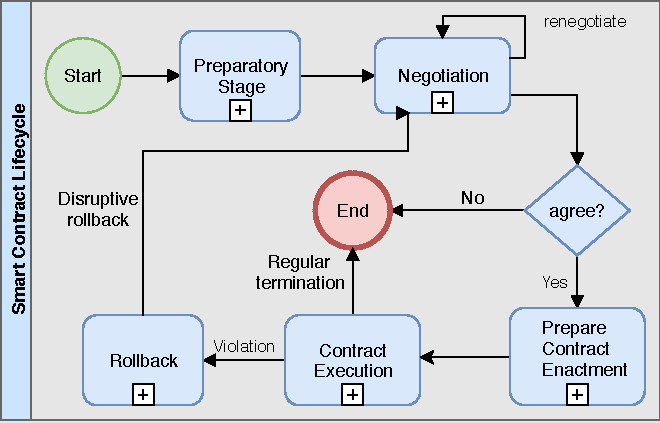
\includegraphics[scale=0.65]{Figures/smart-contract-lifecycle/20180504_smart-contract-lilfefycle.pdf}
				\caption{Smart contract negotiation lifecycle (Based on \cite{qtumWhitepaper}).}	
				\label{fig:smart-contract-lifecycle-management}
			\end{figure}			

			The transportation contract terminates, or expires either after the defined user arrives the final destination, or when the contract is prematurely terminated. Failing to transport the user to the agreed final destination might result in an immediate rollback of the smart contract or invokes some kind of an mediation process that is supervised by a conflict resolution escrow service that is not depicted in this illustration.
	
			The lifecycle presented in Figure~\ref{fig:smart-contract-lifecycle-management} not only cover trading negotiation but rather all kind of contract enactments, also the insurance use case from Section~\ref{s:section-6} that we implement as a prototype. You prepare and negotiate a contract with your insurance company and execute in case you agree on the specifications. That also covers what happens in case you behave correctly, e.g., reward, as well as punishing bad behaviors, e.g., paying a penalty. A serious violation of the contract from any of the involved parties might result in an early termination of the contract or even a rollback.



		%% ----------------------------------------------------------------
		%% ----------------------------------------------------------------	
		
		\subsection{Auction Algorithms}
			\label{ss:auchtion-algorithm}				

			A further important core concept of the Chorus transaction library is to support the exchange and provision of goods on services between entities (V2X). When trading goods and services, the buying and the selling party usually have contrary goals in terms of pricing. The seller's goal is to maximize his/her profits while the buyer tries to minimize the costs. Auctions are a common approach to reach a consensus on a certain price between buyer and seller. We designed two auction algorithms based on the concept of so called Vickrey Auction \cite{moldovanu1998goethe}\cite{vickrey1961counterspeculation}; An algorithm for the scenario with exactly one buyer and one seller, as well as an algorithm that can be used in scenarios with multiple buyers and multiple sellers. Figure~\ref{fig:auction-algorithm-1-1} illustrates one-to-one auctions and Figure~\ref{fig:auction-algorithm-X-X} many-to-many auctions.
			
			During a Vickrey auction, participants exchange sealed bid. Each bidder submits a written and signed bid without knowing the bid of the other participants. In the end, the highest bidder wins but instead of paying the price of this highest bid, the price paid is the second-highest bid. Due to space constraints and the technical nature of this whitepaper we will not cover the economical and game theoretical implications concepts of Vickrey auctions and instead refer the reader to specific supplementary literature, e.g., \cite{ausubel2006lovely}\cite{edelman2007internet}\cite{lucking2000vickrey}\cite{moldovanu1998goethe}\cite{vickrey1961counterspeculation}.

			Figure~\ref{fig:auction-algorithm-1-1} presents a sequence diagram of our one-to-one auction algorithm. We assume that the buyer is not willing to pay more than US\$3, and the seller is not selling for less than US\$2.80. As mentioned in our AOM goal model (Figure~\ref{fig:top-level-aom-goal-model-extended}, speed is one of the non-functional goals of our system - hence, only one auction round is conducted.  Both participants prepare an encrypted (sealed) and signed bid before exchanging the bids. As soon as both participants received the other parties bids, the encryption keys are exchanged as well. Buyer and seller decrypt the bids and compare the offers. Given the case that the buyer offered more than US\$2.80 the auction is successful and due to the second-price rule of Vickrey auctions, the buyer pays US\$2.80 to the seller. In case the buyer offers less than the seller's minimum price the auction ends without a deal.
			
			\begin{figure}
				\centering
				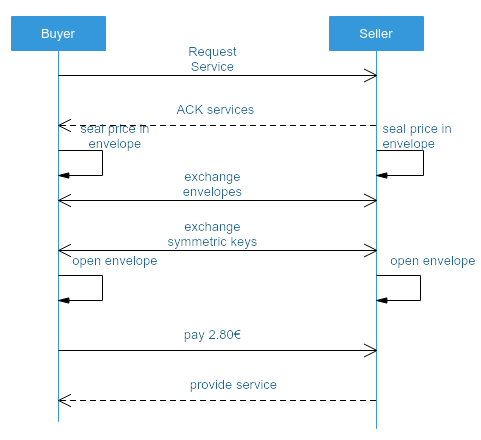
\includegraphics[scale=0.5]{Figures/auction/20180501_auction-aglorithms--1-to-1.png}
				\caption{Chorus auction algorithm - 1 buyer and 1 seller.}	
				\label{fig:auction-algorithm-1-1}
			\end{figure}

			In case multiple buyers and sellers participate in an auction the workflow is very similar as illustrated in Figure~\ref{fig:auction-algorithm-X-X}. We assume a scenario where buyer one is willing to pay a price of US\$1.80, buyer two offers a price of US\$3.20 and buyer three offering US\$3.50. The seller is not selling for less than US\$2.0. Again, we only conduct a single auction round and the buyers as well as the seller all submit their bid in an encrypted and signed envelope that is distributed and send to all registered participants. As soon as all participants received the bids, the encryption keys are exchanged as well and the sealed bids are decrypted. Buyer three wins the auction and pays the seller the price of buyer two that offered US\$3.20.
			\begin{figure}
				\centering
				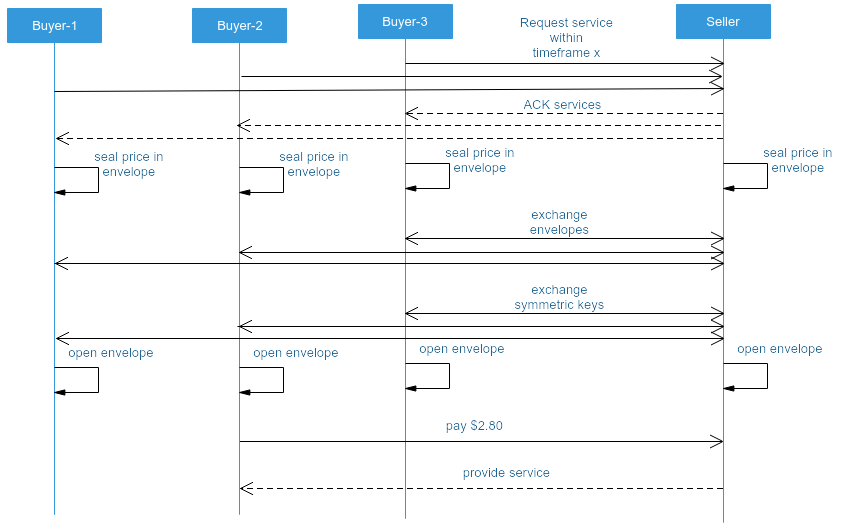
\includegraphics[scale=0.4]{Figures/auction/20180501_auction-aglorithms--X-to-X.png}
				\caption{Chorus auction algorithm - Many buyers and many sellers.}	
				\label{fig:auction-algorithm-X-X}
			\end{figure}			
			In case we have multiple sellers, the sequence diagram is almost identical and the bidding process follows the same procedure. Except in the end, the highest bidder is paying the second highest price to  the seller with the highest minimum price, and so on - as long as the payed price is higher than the matched seller's minimum price.
			 

		%% ----------------------------------------------------------------
		%% ----------------------------------------------------------------	

		\subsection{Token Economics and Value Proposition}
			\label{ss:token-economics}

			\textbf{Work-In-Progress}
			
			%burnable tokens ERC721?\\			
					
		%% ----------------------------------------------------------------
		%% ----------------------------------------------------------------	

	%% ----------------------------------------------------------------
	%% ----------------------------------------------------------------

	\section{Prototype and Feasibility Study}
		\label{s:section-6}	
			
		Chorus Technology developed a prototype to test the feasibility of the V2X platform solution. We decided on a use case where car insurance companies can incentivize good driving behavior of their clients via our platform. Good driving behavior comprises several factors such as: Keeping the distance to the car in front, no aggressive acceleration, no excessive speeding, no hard breaking if not necessary or not using the phone while driving. Not only do these good driving behavior guidelines increase the overall safety of the driver as well as all other road users, they also help to mitigate traffic congestions in urban areas. As a side product, fewer traffic jams also reduce the probability of car accidents which is again in the interest of insurance companies.
		
		The following Section~\ref{ss:protoype-architecture} outlines the architecture and technical details of the prototype, whereas Section~\ref{ss:prototype-incentives} deals with the economics and incentives.
		
%		what is the use case and purpose of our prototype
%		
%		traffic wave fixing as one of the major selling points in the prototype as well as the main product
%		
%		insurance example
%		
%		it is not a library yet - it is a concept prototype
%		

%		
%		- what problem does it solve?		
%		
		%% ----------------------------------------------------------------
		%% ----------------------------------------------------------------	
		
		\subsection{Prototype Architecture}
			\label{ss:protoype-architecture}				

			In order to reduce complexity and speed up the development process of the prototype, we decided to simplify the architecture of the application. As a result, merged the Chorus mobile application (illustrated earlier in Figure~\ref{fig:system-architecture--app}) and the \textit{vehicle} sub-system (presented earlier in Figure~\ref{fig:system-architecture--vehicle}) and only implemented the most basic functionalities of the V2X platform (Figure~\ref{fig:system-architecture--platform}) that is necessary to deploy the prototype. The resulting prototype architecture of our Android application is shown in Figure~\ref{fig:prototype-system-architecture} using a UML component diagram. Due to the simplification and reduced complexity, the illustration is very similar to Figure~\ref{fig:system-architecture--app} except that the Chorus firmware component is now located on the user's mobile phone and manages the good-driving behavior plug-in and also accommodates the necessary blockchain client. We implemented and deployed a smart contract that receives the driving data collected via the smartphone's sensors, e..g, \textbf{add-stuff-here}, stores them on IPFS\footnote{\url{https://ipfs.io/}} and calculates the drivers' score. A score based on the gathered data is calculated for each single ride, as well as a second main score that represents the overall driving behavior based in all previous rides. To ease the integration and reduce development time, we decided to use Infura\footnote{\url{https://infura.io/}} that provides an API with secure, reliable, and scalable access to Ethereum (Rinkeby TestNet) and IPFS. The V2X platform is not shown in Figure~\ref{Bibliography} and we only implemented a rudimentary version of that component, basically focusing on the smart contract functionalities and plug-in interaction and transaction.

			\begin{figure}[H]
				\centering
				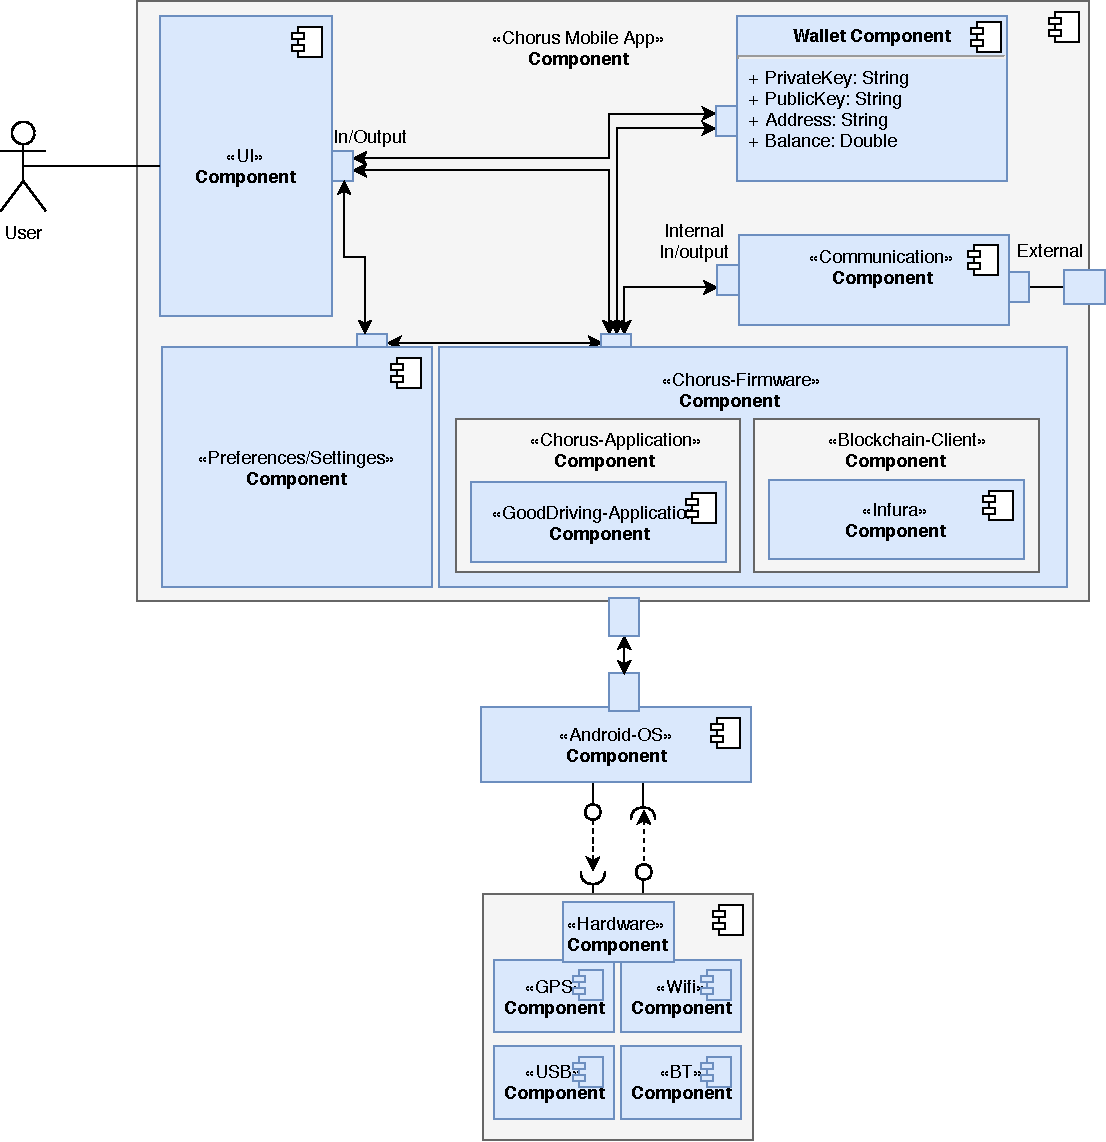
\includegraphics[scale=0.65]{Figures/prototype-architecture/20180509_prototype-architecture-merge.pdf}
				\caption{System architecture of the Chorus prototype.}	
				\label{fig:prototype-system-architecture}
			\end{figure}
			
%			- component diagram
%			- scoring algorithm
%			- tech stack (?)
%			- token
%			- testnet
%			- incentive system

			Currently input data is gathered via the mobile phones build-in hardware sensors and no data is received from the car. Besides vehicle related sensor data such as acceleration and breaking, we also perform localization tasks via hardware in the user's smartphone (GPS, Glonass, etc.). Future version of the Chorus platform may incorporate alternative localization service such as FOAM \cite{foamWhitepaper}. FOAM provides is an open protocol for decentralized geospatial data that aims to to enable their users to build trustworthy consensus-driven map of the world that can be used by any kind of application.


		\subsection{Eco-System and Economics}
			\label{ss:prototype-incentives}
		
			\textbf{Work-In-Progress}		
			
	%		burnable tokens ERC721?\\

					
		%% ----------------------------------------------------------------
		%% ----------------------------------------------------------------	
		
%		\subsection{Evaluation}
%			\label{ss:evaluation}				
%
%			\textbf{Work-In-Progress}
%			
					
		%% ----------------------------------------------------------------
		%% ----------------------------------------------------------------			

	%% ----------------------------------------------------------------
	%% ----------------------------------------------------------------

	\section{Analysis of Related Work}
		\label{s:section-7}	
		
		%Intro

		%% ----------------------------------------------------------------
		%% ----------------------------------------------------------------	
		
%		\subsection{Critical Analysis}
%			\label{ss:critical-analysis}
%							
%			\textbf{Work-In-Progress}		
		
		%% ----------------------------------------------------------------
		%% ----------------------------------------------------------------			
		
%		\subsection{Related Work}
%			\label{ss:competitor-analysis}
			
		In recent time, other project and teams proposed solutions and systems that are related or overlap with the functionalities of our solution. The following Section~\ref{sss:academic-competitors} briefly highlights some academic projects, whereas Section~\ref{sss:non-academic-competitors} outlines competitors from the private sector.

		%% ----------------------------------------------------------------
		%% ----------------------------------------------------------------			

		\subsection{Academic Competitors}
			\label{sss:academic-competitors}
			
			The authors of \cite{leiding2016self} outline a blockchain-based solution for a variety of services within self-managed vehicular ad-hoc networks (VANETs) such as traffic management, toll payment systems, traffic regulation enforcement and more. In \cite{leidingM2M}, the same authors envision a more holistic and abstract machine-to-machine (M2M) economy enabled by a platform that allows trading of goods and service between any kind of machines - ranging from toll road management to automated food  supply- and demand management between fridges and the supermarket and several other scenarios. A special case of this research was independently published by the authors of \cite{sikorski2017blockchain}. They propose and implement a M2M electricity market for chemical industry where energy producers and consumers are trading electricity with each other via a blockchain platform.

		%% ----------------------------------------------------------------
		%% ----------------------------------------------------------------			
			
		\subsection{Non-Academic Competitors}
			\label{sss:non-academic-competitors}

			The alternative blockchain implementation IOTA \cite{iotaWhitepaper} is probably one of the most noticeably known IoT focused blockchains and widely used. IOTA is offering an IoT market place \cite{iotaMarketplace} for IoT devices where sensor data can be bought and sold using blockchain technology, but has no smart contract capabilities and is more a general purpose IoT storage chain than a service provision platform.
			
			Oaken Innovations\footnote{\url{https://www.oakeninnovations.com/}} implemented a prototype of a blockchain-based toll road system \cite{oakenTeslaTollbooth} as well as a blockchain-based water meter application \cite{oakenWaterMeter}. Despite support from different car manufacturers their architecture currently lacks scalability and is dependent on in-vehicle hardware nodes resulting in integration overhead. 
			
			Swarm City\footnote{\url{https://swarm.city/}} is a blockchain-based and decentralized commerce platform work running on the Ethereum network \cite{swarmWhitepaper1}\cite{swarmWhitepaper2}. It has a built in marketplace and reputation system and focuses on enabling transactions between humans without third-party interaction. By putting all computation logic on the Ethereum blockchain, the scalability and computation power of Swarm City couple dApps is rather limited and not suitable to be applied in the context of VANETs.

			Flying Carpet\footnote{\url{http://www.flyingcarpet.network/}} is a blockchain-based, decentralized and autonomous P2P transportation network. The project is in its early stages and the MVP use case focuses on decentralized charging and docking station for drones or UAVs.

			The DAV project \footnote{\url{https://dav.network/}} outlines a solution that allows vehicles to discover, communicate and transact with one another using cryptocurrencies \cite{davWhitepaper}. Their use cases are similar to some of the Chorus examples described earlier, but rather than providing a coherent transaction layer protocol with an integrable library, they focus on use case based solutions.
			
			In 2018, the Ford Motor Company got a patent approval for a traffic marshaling via a blockchain system \cite{macneille2018vehicle} that is similar to the ideas described in the academic papers of \cite{leiding2016self}. Despite having a patent, the solution is focused on a single use case and not suitable to be adapted to a general service provision platform for VANETs. 

			XAIN\footnote{\url{https://www.xain.io/}} created and implemented their own Ethereum-based low-energy blockchain with a customized proof-of-work algorithm \cite{xainWhitepaper}. Despite having worked on a jointed project with car manufacturer Porsche, their vision and longterm strategy remains unclear.

			Slock.it\footnote{\url{https://slock.it/}} is another project focusing on specific use case rather than a general solution concept. They are working on a universal sharing network that enables anyone to rent, sell or share their property without a middleman \cite{slockWhitepaper}. Even though their solution potentially also includes cars, they do not consider any other of the use cases presented in this whitepaper.

			DOVU\footnote{\url{https://dovu.io/}} \cite{dovuWhitepaper} is currently testing a system for drivers to log mileage in leased or borrowed vehicles in the UK. In general, DOVU is working on a vehicle-focused ubiquitous rewards system that can be used in various scenarios of VANETs.
			
			Weeve\footnote{\url{https://weeve.network/}} \cite{weeveWhitepaper}
		
		
		%% ----------------------------------------------------------------
		%% ----------------------------------------------------------------					
	
	%% ----------------------------------------------------------------
	%% ----------------------------------------------------------------

	\section{Conclusion and Future Work}
		\label{s:section-8}	

		This whitepaper presents the Chorus Technology blockchain-based transaction and interaction layer for (semi)-autonomous vehicles that enables a V2X platform for goods and services. We outline and describe the technical foundations of this new economy, the longterm vision and benefits as well as the different use cases and scenarios of V2X transactions and interactions, e.g., vehicle-to-vehicle (V2V), vehicle-to-human (V2H), or vehicle-to-infrastructure (V2I).
		
		Based on the use cases and scenarios we identify the requirements and criteria that a blockchain-based V2X transaction and interaction layer protocol must satisfy. With respect to functional and non-functional requirements, Chorus aims to develop a blockchain- as well as manufacturer agnostic and interoperable V2X platform that enables interaction and transaction between participating entities and a plug-in interface for external applications.
		Subsequently, we derive the service-oriented architecture of the our system based on the identified requirements and goals. We present the system architecture using technology-agnostic UML-component and sequence diagrams that detail the system’s main components and communication interfaces. In order to ensure widespread adoption, special focus will be given in the future to the API design and library integration for car manufacturers.
		
		A core element of many of the Chorus use cases is smart contract-based negotiation and contract enactment between
		entities that are the result of collaborating tasks and subprocesses. On an abstract level, most of the use cases presented in this paper follow a similar workflow on the smart-contract level. Hence, we decided to integrate an abstract smart contract negotiation lifecycle that we describe. The lifecycle is divided into the different stages (preparatory, negotiation, contract execution, rollback and contract expiry stage) that we explain in detail. Furthermore, we designed two auction algorithms for the V2X economy that allow to reach an efficient consensus on a certain price between buyer and seller. Our auction algorithms are based on the concept of so called Vickrey Auction, and we envisioned one algorithm for one-to-one interaction as well as a second workflow for scenarios with multiple buyers and sellers. Finally, we present the Chorus token value proposition and the surrounding token economy eco-system that fuels the V2X platform.
		
		Next, we present a Chorus prototype implementation. We demonstrate how our protocol can help mitigating traffic congestions and at the same time provides a mean to car insurance companies to incentivize their customers to practice good driving behavior. 	
		
		Future releases will focus on the longterm vision of Chorus Technology and the development of the abstract transaction and interaction layer as well as the API and library integration. Besides that, we will also continue to focus on further research aspects of the upcoming V2X economy that will facilitate future developments of Chorus Technology.

	%% ----------------------------------------------------------------
	%% ----------------------------------------------------------------


	\label{Bibliography}
	\bibliographystyle{splncs03}
	\bibliography{Bibliography}
	
	%% ----------------------------------------------------------------
	%% ----------------------------------------------------------------	



	%
\end{document}


